

\chapter{Introduction}


\section{The Problem}


\begin{changemargin}{4em}{4em} 

\vspace{1em}

    \textit{The soles of our boots wear thin, but the soles of feet grow thick, the more we walk upon them.} \\[4pt]
    \hspace*{16.5em} ---D'Arcy Thompson (1917)
    
\vspace{1em}
    
    
\end{changemargin}


\noindent
This thesis has as its basis the fact that organisms are at once autonomous and adaptive systems, and robots are not.

By far the most commercially successful autonomous robot to date is the self-driving vacuum: the Roomba. 
Roombas are autonomous but non-adaptive systems.
Mine is routinely defeated by the same long shoelace, which it eats and coils around its spinning brush and wheels until they grind to a halt.
An adaptive robot would sense that something had gone awry, and respond by altering its behavior so as to preserve its functionality.
That is, an adaptive robot would change so as to remain the same.


Autonomous adaptive machines could provide immense social utility.
They could be used to patrol, remediate, and protect our bodies and our planet. 
They could help us build new infrastructure,
here on Earth and in space,
and technological artifacts
% at the scale of planets.
far beyond the size scales we have achieved thus far.
If successful, an increasingly dense, rich, and empowering web of human-robot interaction would be realized.
Robots would no longer simply serve as workers or mere extensions of the human mind, like most other technologies.
They would become our peers.
However, this vision will only be possible if our robot symbionts are both autonomous and adaptive, like every organism on Earth.


One could argue that the essential difference between organisms and current robots is that organisms are \textit{protean} systems:
Organisms, like Proteus,
% of Greek mythology, 
are constantly forming and reforming.
All conventional robots to date, on the other hand, are deployed with a fixed morphology which does not change during operation.



\section{Contributions}
\label{sec:contributions}


\begin{changemargin}{4em}{4em} 

\vspace{1em}

    \textit{Proteus will seek to foil you by taking the shape of every creature that moves on earth, and of water and of portentous fire; but you must hold him unflinchingly and you must press the harder.} \\[4pt]
    \hspace*{16.5em} ---Homer (C8th B.C.) 
    
\vspace{1em}
    
    
\end{changemargin}

\noindent
In the pages that follow, I will demonstrate the utility of increasingly protean machines through a series of evolutionary robotics experiments that were performed over the course of four years, during my time as a Ph.D.~student at the University of Vermont \mbox{(2016-2020)}.
% This section is a sketch of the main contributions.
Seven key benefits were uncovered and scrutinized:

\begin{enumerate}

    \item Protean body plans permit continual learning \cite{thrun1995lifelong} and open-ended evolution 
    \cite{%
    %bedau1998classification,
    maley1999four} 
    in machines with open-loop or static control systems.
    This is possible because of hardware revisions, 
    % (to shape, structure, and/or material properties) 
    persisting over extended periods of 
    % developmental 
    time, that cause the same sequence of actions to generate different behaviors (chapters 2, 3, 6 and 7).
    This is important because controllers are often complex software, finely tuned prior to deployment and difficult to re-specify in the field.

    \item Protean body plans introduce smaller and thus safer mutations \cite{lehman2018safe}, whose behavioral deflection manifests temporarily during operation, rather than permanently from deployment (chapter 3).
    Evolution can then lengthen the time intervals containing superior traits and reduce the intervals of inferior traits.
    This allows evolution to surgically revise morphology with a pair of tweezers, if you will, rather than a sledgehammer.


    
    \item Protean body plans smooth the search space evolution operates in via the Baldwin effect (chapters 3 and 4).
    This effect is outlined in Figs.~\ref{fig:baldwin2d} and \ref{fig:baldwin3d}.
    In brief, the flexibility of a protean feature
    (e.g.~skin thickness) allows evolution to sweep through design space along a line of development rather than sampling a single point.
    Development can then be incrementally canalized about a good static setting (e.g.~calluses).
    This gradual homing-in process is hastened by natural selection,
    and eventually supplanted by the genetic determination of the feature 
    % which in previous generations needed to be rediscovered by development. 
    (e.g.~embryonic calluses).
    % that in previous generations was protean.
    %  that would otherwise be need to be earned through interaction with the environment
    This well-studied phenomenon is revisited with a twist:
    physically embodied robots, rather than an abstract control system.
    This distinction is important because it grounds hypotheses in the constraints and opportunities afforded by the physical world.
    
    \item Protean body plans promote (the canalization of) permissive body plans robust to control changes (chapter 4).
    It is much easier to train a control policy within a permissive body. 
    % Evolution discovers body plans robust to control changes, these body plans become genetically assimilated, yet controllers for these agents are not assimilated.
    This exposed a previously unknown detail about the Baldwin effect: instead of all useful traits becoming genetically assimilated, only traits that render the agent robust to changes in other traits become assimilated. 
    % This exposed the previously unknown phenomenon of differential canalization reported here.
    I refer to this as \textit{differential canalization}.
    
    \item Protean body plans foster ``zero-shot'' generalization (on the very first try, without adjustment) to fabrication errors (chapter 5).
    The amount of generalization in canalized (previously protean but now morphologically-static) machines was found to depend on the kinds of interoceptive signals used to guide their morphological change during optimization.
    
    \item Protean body plans amplify robustness to damage (chapter 6).
    This is because a sufficiently deformable body can in some cases morph to ``resonate'' with an existing control policy---tuned prior to damage---to regenerate behavioral competence (not necessarily by reforming the original body shape).
    This allows protean machines to recover functionality after ``deep insult'', such as removal of all limbs, or being cut in half.
    
    \item Protean body plans regulate building blocks that exhibit unpredictable behavior, such as cardiomyocytes (heart muscle) when reorganized into novel structures in vitro (chapter 7).
    Structural evolution in silico can yield an appropriate static morphology that denoises and stabilizes even completely random control policies.
    Under certain constraints, such robust designs can be built as new organisms, designed by a computer, that are by virtue of their living cells inherently protean.
    
    % \item Protean body plans steer collectives of autonomous agents, such as swarms of computer-designed organisms, toward desired system-level outcomes (e.g.~kinematic self-replication) and away from emergent unintended consequences.
    
\end{enumerate}

\vspace{1em}

\noindent
In addition to these seven intellectual contributions, 
two new platforms for constructing physical protean machines were developed as part of this thesis:

\begin{enumerate}
    \item \textit{Voxcraft.} A modular soft robot design and construction kit (used in chapters 2 and 6), 
    voxcraft is open-source, safe, inexpensive, and simple.
    The goal of voxcraft is threefold:
    Lower the barrier of entry to soft robotics for non-experts,
    facilitate new research in evolutionary robotics,
    and simplify the replication of those studies.
    More information can be found at:
    \href{https://voxcraft.github.io/}{\color{blue}\texttt{voxcraft.github.io}}
    
    % \vspace{4pt}
    
    \item \textit{Reconfigurable Organisms.} Chapter 7 reprises the 2020 study that introduced the first computer-designed organisms: xenobots.
    AI methods automatically design diverse candidate lifeforms in silico to perform some desired function, and transferable designs are then created using a cell-based construction toolkit to realize living systems with the predicted behaviors. 
    % Frog cells, configured by natural selection to become frogs, were reconfigured by AI to create new forms and functions. 
    % The aggregated cells of the resulting computer-designed organism (CDO) can also be disassociated and reconfigured to form a new CDO.
    More information can be found at: \href{https://cdorgs.github.io/}{\color{blue}\texttt{cdorgs.github.io}}

\end{enumerate}




\newpage
\section{Ontology}
\label{sec:ontology}

\begin{changemargin}{4em}{4em} 

\vspace{1em}

    \textit{A ``system'' is a set of variables sufficiently isolated to stay dis-cassable while we discuss it.} \\[4pt]
    \hspace*{16.5em} ---W.~Ross Ashby
    
\vspace{1em}
    
    
\end{changemargin}

\noindent
In the chapters that follow, we will incrementally liberate different physical attributes of a robot's design so that they may vary during operation.
This section 
% (roughly) 
defines each such variable, 
how they relate to each other (Fig.~\ref{fig:taxonomy}), 
as well as the different time scales in which they may change.
The definitions are necessarily fuzzy around the edges, idealized, stipulative, and include (at least) one category mistake---but they will be precise enough to be useful.
% Later, when more exact concepts have been developed (e.g.~how physics is simulated), it will be possible to state the ontology more precisely.% (chapter 6).


\begin{enumerate}

    \item \textbf{Time.} It will be convenient to define $\{T\in\mathbb{N} \,|\, T>0\}$, for evolutionary (phylogenetic) time, and $\{t\in\mathbb{R} \,|\, t>0\}$, for developmental (ontogentic) time.
    Time is strictly positive, with $t$ nested inside of $T$.
    Nested inside of $t$, is another timescale---that of physiological functioning (e.g.~the beating of a heart) and behavior (e.g.~the cycle of a gait):
    ``here and now'' as \citet{pfeifer2006body} put it.
    Time is of course relative to an observer---and there are nested observers.
    Here-and-now is minutes for a squirrel burying acorns, seconds for a dog chasing the squirrel, milliseconds for a racing heart, microseconds for its gated ion channels, pico- or femtoseconds for its vibrating molecular bonds.
    We can denote these finer timescales $\theta_1, \theta_2, \ldots$
    if you wish.
    But that won't be strictly necessary.
    
    $T$ and $t$ are enough to describe the basic algorithm of evolution in time.
    For the entire $n$-th generation of evolution, $T=n$ as a population of designs develop and behave for $\tau$ seconds during ontogeny: an evaluation period over $t\in(0, \tau)$.
    The worst designs are culled and replaced by noisy copies of the survivors.
    $T$ is incremented by one, $t$ starts over at 0, and generation $n+1$ begins.
    
    % Let $T\in\mathbb{N}=G$ be the current generation and $t\in\mathbb{R}=d$ be a moment in a robot's life.
    % To measure an in life process we define $p:\alpha\rightarrow\theta$ where $\theta$ may be $\mathbb{R}$, $\mathbb{N}$, or any other suitable set and $p(t)$ a function of ontogenetic time.
    % Example: Heartbeat
    % $p(t)=\sin(t)*\sin(t+1.5)$
    
    % Time was the first term to be defined because it affects the robot in a fundamentally different way than other variables.
    Note that this neat organization of timescales will
    later be turned inside out when designs are evolved without development in silico, and then built as organisms that develop but do not evolve and cannot reproduce in vivo.
    
    \item \textbf{Material.} Embodied systems are made out of physical matter
    with mechanical properties: 
    mass, density, friction,
    stickiness,
    viscosity,
    elasticity, plasticity,
    stability,
    strengths and limits.
    These 
    properties determine the system's passive dynamics and can thus streamline or frustrate the evolution of adaptive behavior.
    Material properties can be heterogeneously distributed across a robot's body, and in some experiments, 
    can change non-uniformly across the robot's body, in both evolutionary and developmental time.
    
    %
    \begin{figure}[H]
    \begin{minipage}[t]{0.47\linewidth}
        \centering
        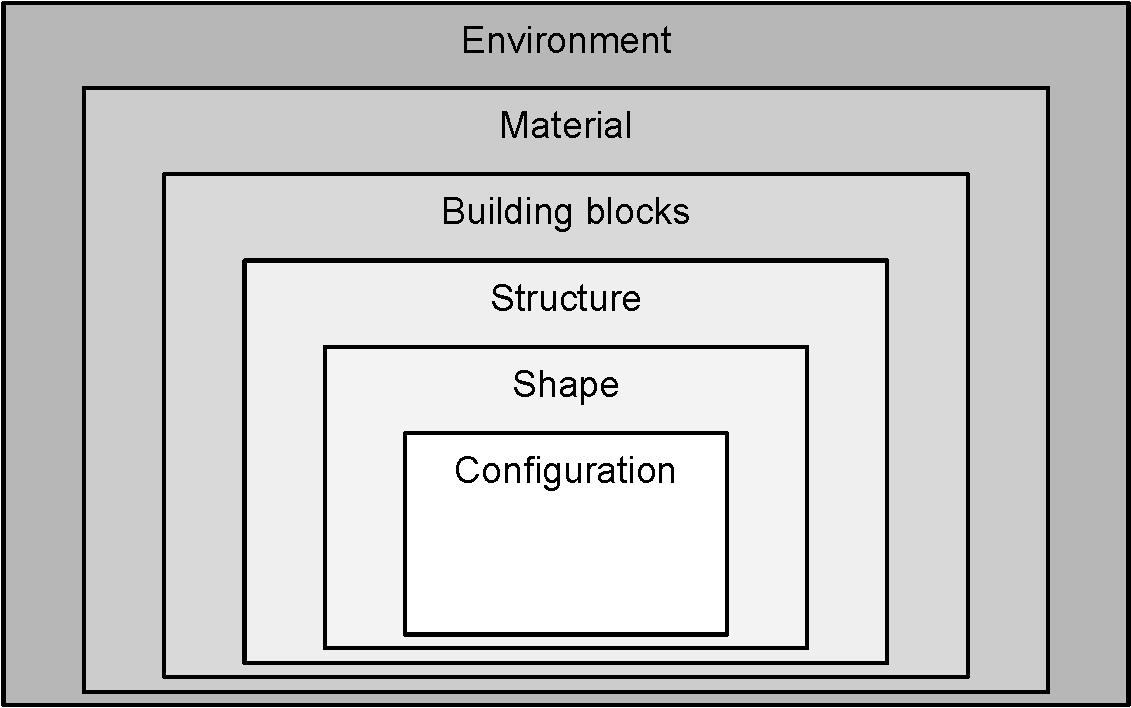
\includegraphics[width=\linewidth]{fig/taxonomy}
        \caption{\label{fig:taxonomy}\textbf{Taxonomy of a robot's state.} 
        The environment is a source of innumerable variables that can affect the robot.
        Within the environment there are materials from which building blocks may be fashioned.
        Building blocks of material are connected together to form a structure.
        A given structure can be deformed into various resting shapes.
        Configurations deflect the robot's structure about a resting shape, with elastic strain energy proportional to the deflection.
        }
    \end{minipage}
    \hfill
    \begin{minipage}[t]{0.47\linewidth}
        \centering
        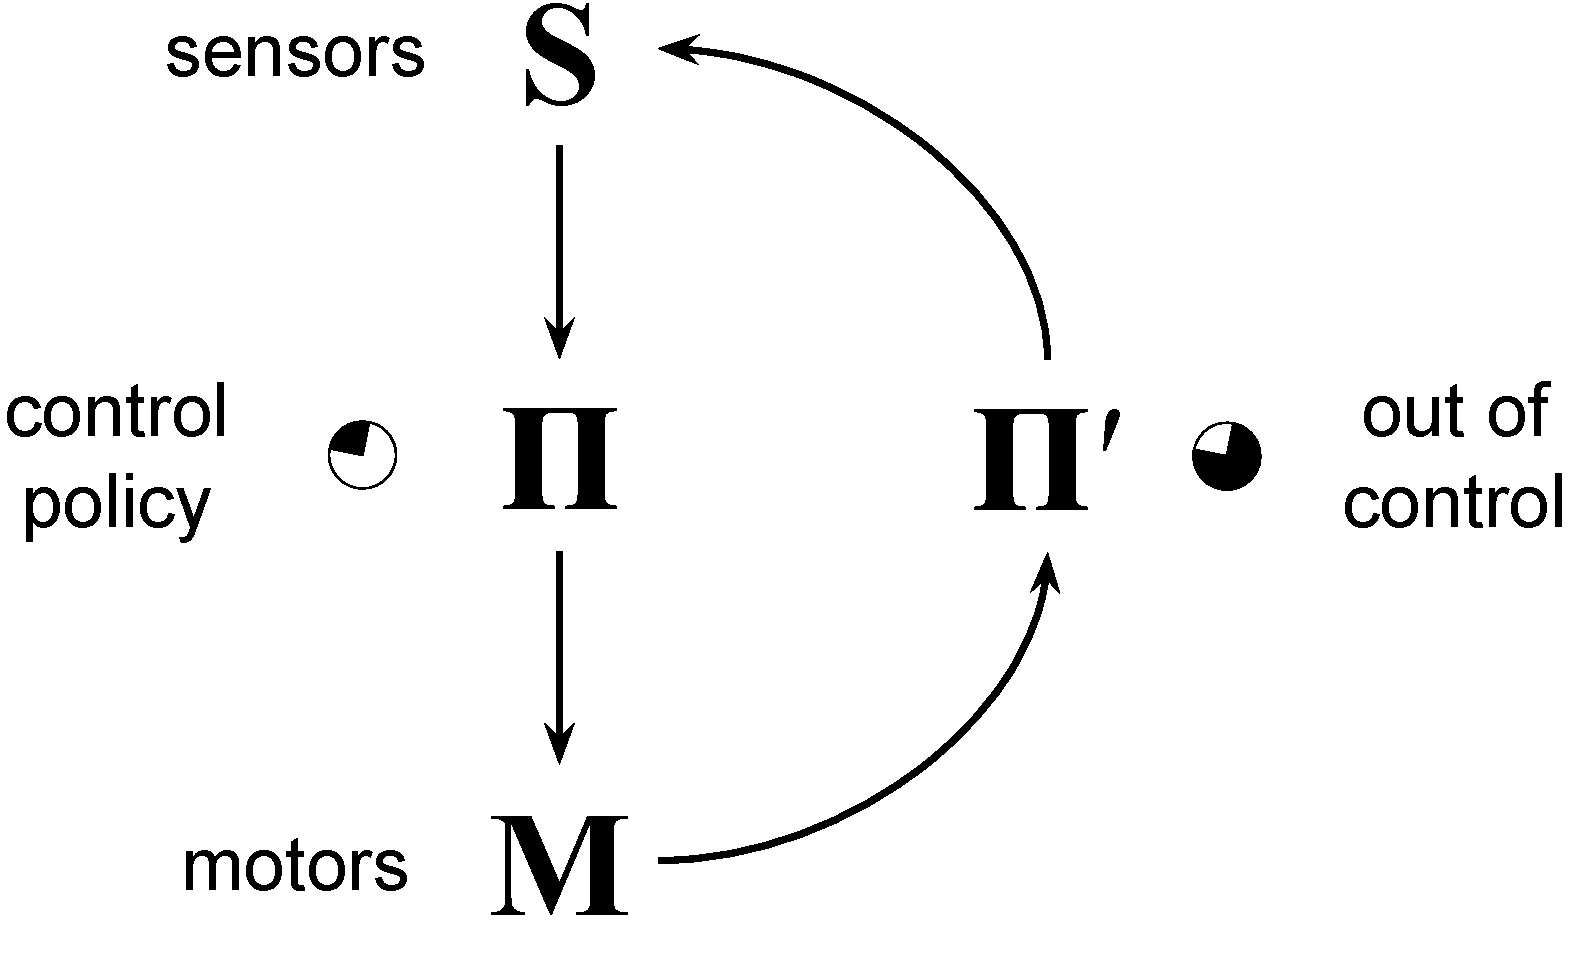
\includegraphics[width=\linewidth]{fig/sensor-policy-motor.pdf}
        \caption{\label{fig:policy}\textbf{Functional decomposition of state.} A set of sensors {\rm\textbf{S}} are input to a policy $\mathbf{\Pi}$ which controls a set of motors {\rm\textbf{M}}.
        Motors push against the world $\mathbf{\Pi'}$, sensors feel the world push back.
        % Some attributes of the robot can be purposefully varied by the robot in reaction to its sensor readings: they are in $\mathbf{\Pi}$. 
        % All of the other variables due to the robot's body or environment that are varied by $\mathbf{\Pi}$, fall into $\mathbf{\Pi'}$: they are ``out of control''.
        Traditionally, a robot's structure, shape and material properties are not varied by $\mathbf{\Pi}$: they are ``out of control''.
        They are, from the perspective of $\mathbf{\Pi}$, part of the environment.
        This homuncular dissection is ubiquitous in robotics, and often useful for analyzing and predicting behavior.
        }
    \end{minipage}
    \end{figure}
    %
    
    \item \textbf{Building block.} 
    The smallest constituent unit of material that constitutes a robot.
    A block can be a passive slab of raw material,
    or it can itself be composed
    of functional subcomponents, circuitry, sensors and motors.
    Wherever possible, the building blocks will be voxels: congruent cubes that attach face to face to form a structure, known formally as a polycube.
    In computer-designed organsims, however, the building blocks are biological cells: de/ciliated ectoderm and cardiomyocytes.
    
    
    \item \textbf{Structure.} The contiguous topological arrangement and coupling of building blocks.
    % More concretely, the number and placement of sensors, motors, mechanical degrees of freedom, and the framework linking them together.
    The space of possible structures that can be built out of a pile of voxels---the set of polycubes---and the duplicates that result when these structures are translated, rotated or reflected---are enumerable.
    This simplifying constraint biases evolution toward buildable structures (rather than tangled balls of particles) and it makes it easier for any humans in the loop to think about the design space: it's just (squishy and sometimes moist) Lego bricks that can attach on all sides (not just dorsoventrally).
    % 
    % The number of unique behaviors too can be estimated.
    % For example a tortoise robot that walks in straight line (under open-loop control) that is spun about its sagittal plane will simply move in a different direction.
    % But flipped onto its shell (rotated 180$^{\circ}$~about its transverse plane) the robot will struggle to generate forward movement.
    
    
    \item \textbf{Shape.} Plastic deformations and folding in the building blocks of a given structure, which persist after stresses have been removed.
    Or, elastic deformations that are held relatively constant under stress, within some interval of developmental time, during a sequence of configurations (definition 6) (e.g.~as the leg moves from point to point).
    Shape change can adjust the robot's posture, volume, mass distribution, number/placement of limbs, storage/release of elastic strain energy, surface contact geometry and tribology, during behavior.
    % There are numerous mechanisms of shape change currently avaible to robots: pneumatic \cite{hawkes2017soft}, thermal, magnetic \cite{ze2019magnetic}, mechanical \cite{felton2014method}, chemical \cite{gladman2016biomimetic},
    
    \begin{figure}[H]
        \centering
        \vspace{-2pt}
        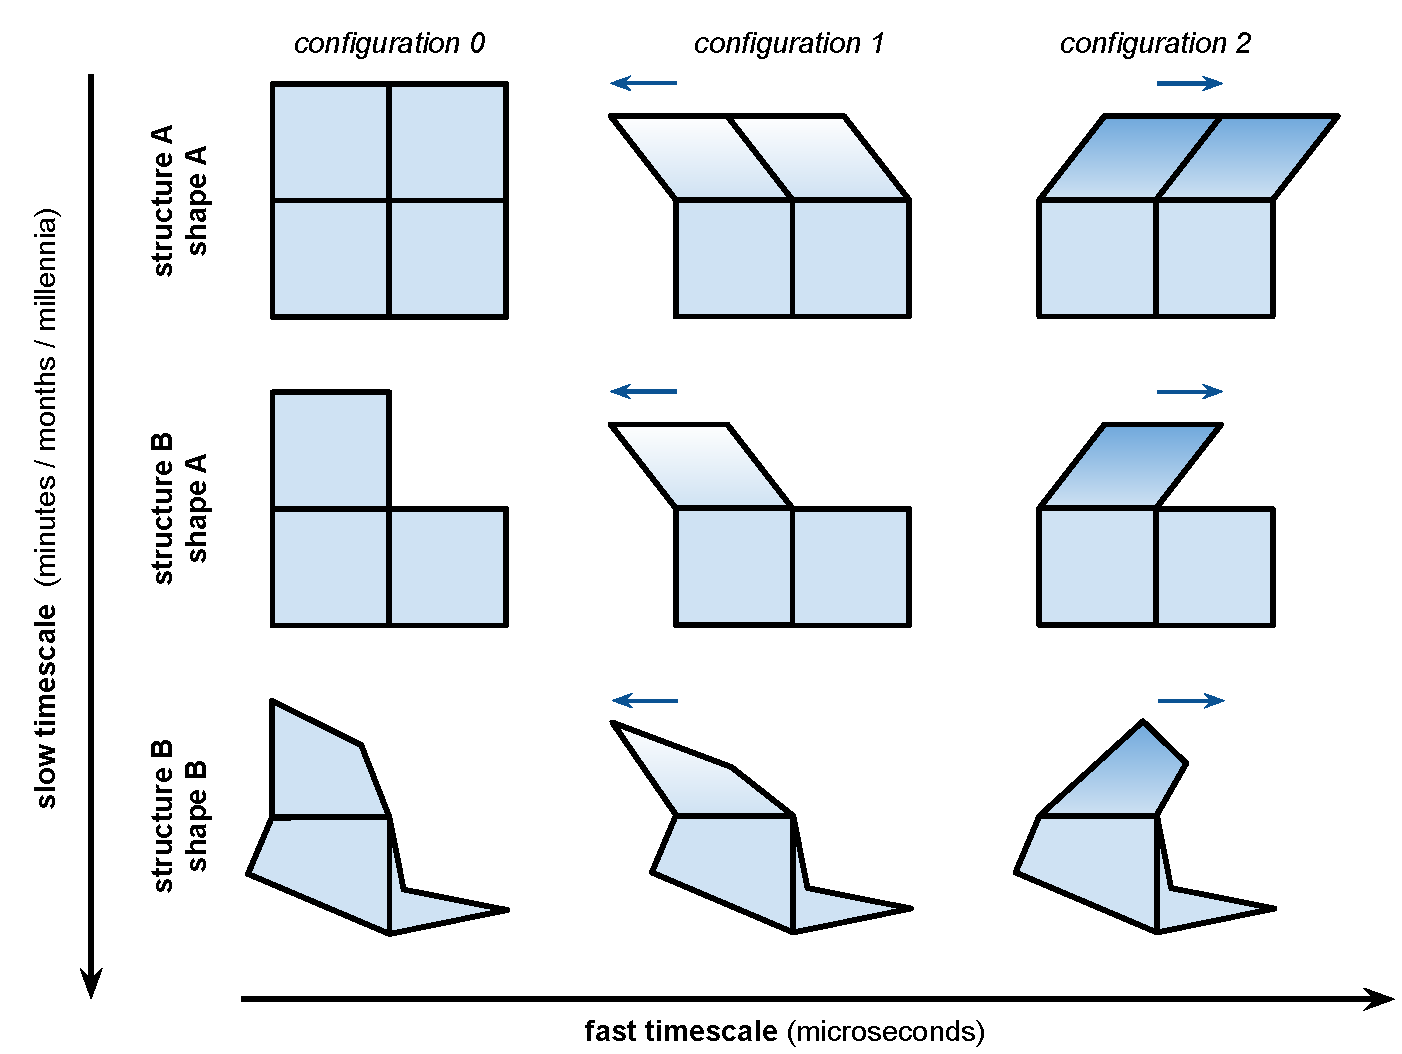
\includegraphics[width=0.9\linewidth]{fig/ontology.pdf}
        \caption{%
        \textbf{Changes of geometry in time.}
        \textbf{By row, top to bottom:}
        A 2-by-2 grid of building blocks is generated (structure A).
        Each block has squarish resting shape (shape A) and identical material properties.
        The material details---%
        and how they might change over time---%
        are not depicted.
        A change in structure occurs when one of the blocks is subtracted from the body plan (structure B).
        Later, changes to the local volume and curvature of each block deform the overall geometry (shape B) without adding, removing or reorganizing the blocks (structure B).
        \textbf{By column, left to right:}
        The body at rest (configuration 0).
        When behaving, dorsal blocks are rapidly shifted back and forth, to the left (configuration 1) and to the right (configuration 2).
        Active blocks are shaded in proportion to their relative displacement due to configuration: lighter when angled to the left, and darker when angled to the right.
        \label{fig:ontology}%
        }
        % \vspace{-6pt}
    \end{figure}
    
    \item \textbf{Configuration.}
    The relative displacement, orientation, and elastic deformation of a robot's structure---%
    away from its current resting shape---% 
    during ontogeny.
    When the robot relaxes, it returns to its resting shape.
    For example, a spherical robot could deform to generate four limbs (shape change) and then move those limbs back and forth to gallop across flat terrain (configuration change).
    Later, the robot could extrude five clawed fingers at the end of each of its limbs.
    By moving its limbs and fingers and torso in a different pattern, it climbs a tree, and swings from branch to branch.
    As the robot travels through the different configurations of running or climbing or swinging, its body will stretch and contort about its root shape.
    
    % By elongating the robots arms, 
    % Gibbons are very good brachiators because their elongated arms enable them to easily swing and grasp on to branches
    
    For a protean machine that can intentionally change both shape and configuration, the distinction between the two becomes somewhat arbitrary.
    Are they not both simply ``actuation''?
    This distinction is most secure, I believe, in terms of the time scales on which processes of shape change 
    % (development) 
    and configuration change 
    % (behavior) 
    occur naturally.
    An amorphous blob could in principle continuously morph as a form of locomotion, rendering its ``configuration'' and ``shape'' equivalent.
    In nature, however, there is modularity: an underlying anatomical shape that is developing yet persists as the organism behaves (Fig~\ref{fig:ontology}).
    
    
    
    \item \textbf{Environment.}
    Variables whose changes affect the robot, 
    and variables which are changed by the robot's actions.
    This definition, adopted from \citet{ashby1952design}, is intentionally broad, encompassing an infinitude of inanimate objects and forces, 
    properties of the surrounding medium,
    the terrain,
    as well as other robots and living systems around and inside the robot.
    
    \item \textbf{State.}
    A robot's environment, configuration, shape, structure and material properties, taken together, at any moment in ontogeny $0<t<\tau$.
    
    
    \item \textbf{Controller.}
    When thinking about robots, it is sometimes useful to define ``controller'' as a separate entity---%
    a ``policy'' \cite{sutton2018reinforcement}
    that steers the robot along a ``line of ontogeny'': a succession of states.
    This is particularly helpful when dealing with electronics and software that is---for good reason---abstracted far away from the details of transistors and ions and sensorimotor circuits.
    % Why did the robot just do a backflip?
    % Ah, I see, line 458: 
    % \begin{changemargin}{2em}{2em} 
    % \small
    % \texttt{%
    % 457: \dots \\
    % 458: if (anteriorUltrasonicSensor > 0) \{ doBackFlip(); \} \\
    % 459: \dots
    % }
    % \end{changemargin}
    % homunculus
    % By adopting ``policies for'' backflipping, climbing a tree, and so on, we can accurately predict and influence a robot's behavior, without working out the specific physical laws
    % of a complex system by ascribing ``beliefs'' and ``desires'' to its actions---by taking the intentional stance 
    % \cite{dennett1989intentional}.
    % This begs the question as to \textit{where} in the robot such desires could inhere?
    % This begs the question as to where in the robot the policy---this ``desire'' to backflip---inheres.
    But we must remind ourselves that this is, in fact, a categorical error \cite{dreyfus1967computers,harvey2000robotics,pfeifer2006body}.
    
    Without invoking a \textit{Deus ex machina}, a line of ontogeny can only be formed by the robot's state and the condition of its immediate surroundings.
    Decomposing state into modules that on one hand ``steer'' and on the other ``are steered'', is an example of what \citet{bennett2003philosophical} call a mereological\footnote{%
    From the Greek $\mu\acute{\varepsilon}\rho{o}\varsigma$ % μέρος 
    \textit{meros}: ``a part, a fraction''.
    } 
    fallacy (e.g.~``brains predict'' \cite{clark2013whatever}).
    Thus ``controller'' is formally identical (isomorphic) to ``state'' and redundant in our ontology.
    But it is nevertheless
    % , lamentably, 
    useful (Fig.~\ref{fig:policy}).
    
    
    \item \textbf{Field.}
    % We have already use the concept of a ``change of behavior'', as when the robot transitioned from running to climbing.
    % Yet the behavior is itself a sequence of changes (e.g.~as the leg moves from point to point).
    Borrowing yet another page from Ashby's book, a ``field'' is defined as ``the phase-space containing all the lines of [ontogeny] found by releasing the system from all possible initial states in a particular set of surrounding conditions.''
    We can now see ``behaviors'' as attractor states in the field of a robot arising from interactions among configuration, shape, structure, material properties, 
    controller 
    and environment.

    When different variables of a robot change on different timescales, slower moving variables define a subfield through which lines of faster moving variables may unfold.
    % From the space of all logically possible genomes
    % Evolution selects from the space of possible genomes, constraining the field of possible ontogenies.
    If a set of variables is fixed, the lines of ontogeny run in a sub-space orthogonal to the axes (Fig.~\ref{fig:ashbyInactiveVars}).
    
    Reconsider the example of limb growth in an initially spherical robot.
    The field 
    surrounding 
    % of
    an actuated sphere turns almost all lines of configuration change into rolling behavior.
    However, by stretching a few physical attributes past a critical point,
    % new configurations became possible and 
    the robot found itself in a new field, capable of a previously unreachable behavior: brachiation (Fig.~\ref{fig:ashbyStepMech}).
    
    
    
 
    
    % The robot from our practical example above, traveled through one line of configurations while galloping, and another line while climbing.
    
    %  A controller steers the robot as best it can through a line of configuration/shape/structure/material changes in its field (possible ways of developing/behaving).
    
    % Different controllers will alter the field lines of behavior/development
    
    % At different locomotion speeds, different gaits (patterns of leg movement) will be more efficient and more ``comfortable'' for the robot.
    % A gait is an example of a line of configuration changes in the phase-space of all possible configurations (the configuration ``field'') of the given structure, shape and material.
    % Switching gaits is an example of a change in 
    
    % may fall into during locomotion across solid ground


\end{enumerate}

% \vspace{-8pt}

\begin{figure}[H]
    \begin{minipage}[t]{0.47\linewidth}
        \centering
        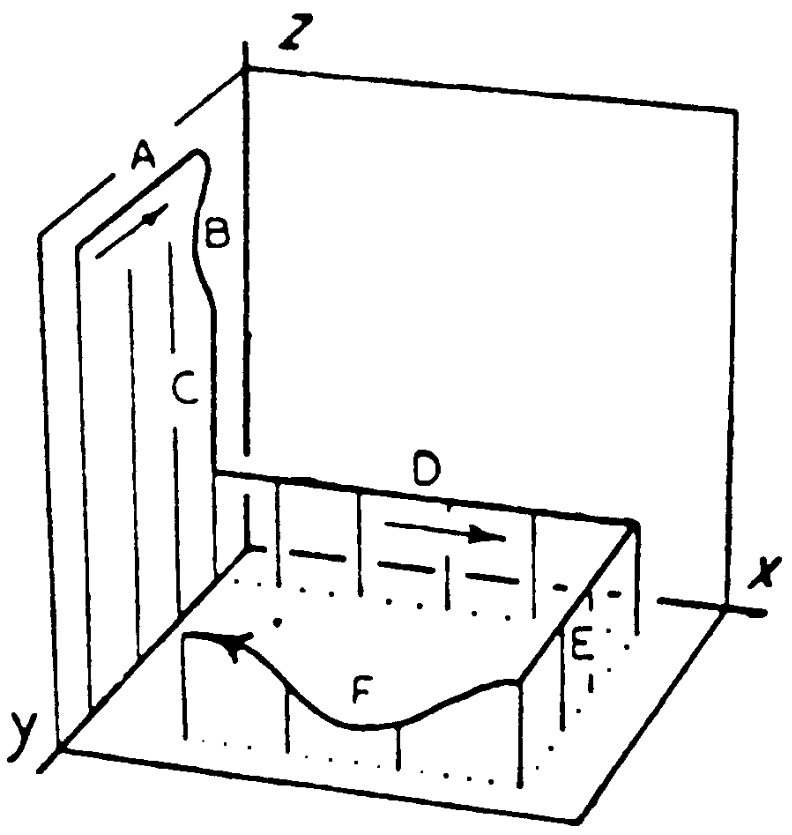
\includegraphics[width=0.65\linewidth]{fig/Ashby12-18-1.png}
        \captionof{figure}{%
        \label{fig:ashbyInactiveVars}
        \citet{ashby1952design} illustrated how inactive variables restrict the active ones to an orthogonal sub-space:
        ``In the different stages the active variables are: $A$, $y$; $B$, $y$ and $z$; $C$, $z$; $D$ $x$; $E$ $y$; $F$ $x$ and $z$.''
        Variables can be practically inactive in relation to those that change on a much faster time scale.%
        }
    \end{minipage}\hfill
    \begin{minipage}[t]{0.47\linewidth}
        \centering
        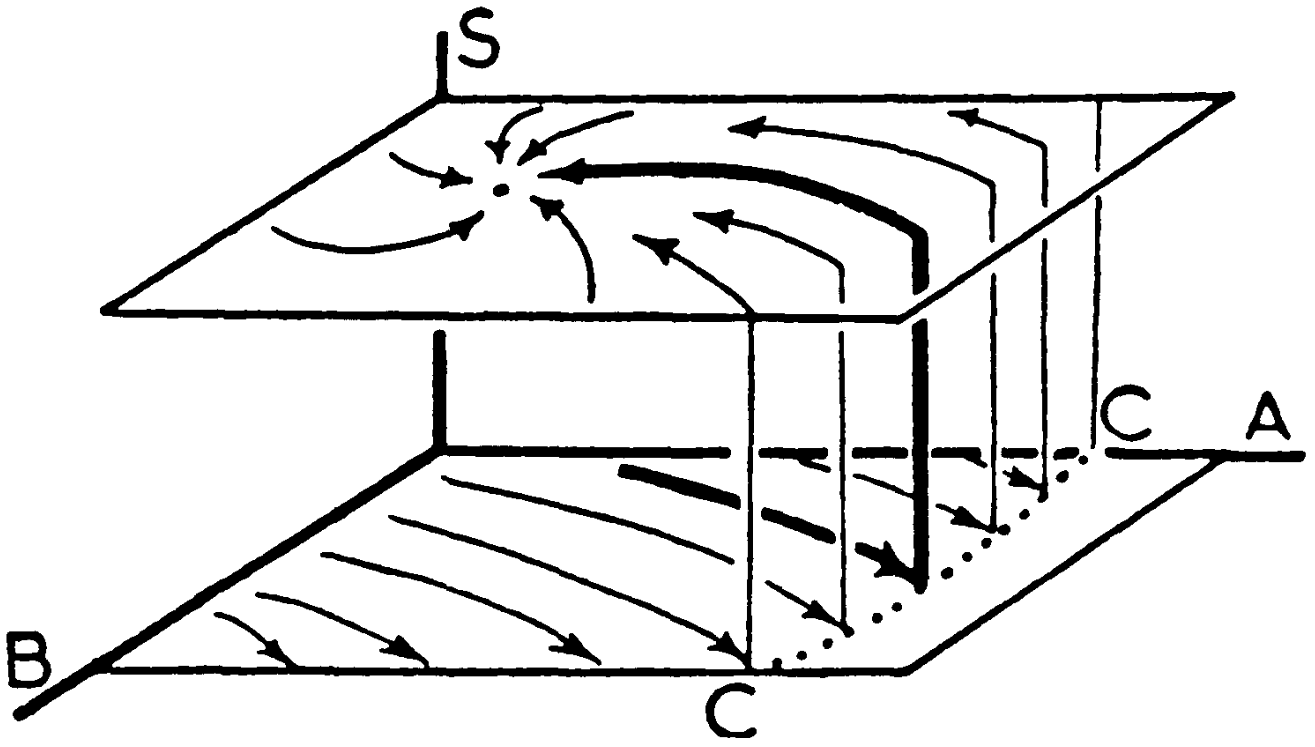
\includegraphics[width=0.9\linewidth]{fig/Ashby7-20-1.png}
        \captionof{figure}{%
        \label{fig:ashbyStepMech}
        In describing variables due to step-mechanisms ($S$),
        \citet{ashby1952design} made clear how a system could be pushed onto new fields through critical states (from $C$ to $C$).
        %
        % ``Field of a state-determined system of three variables, of which $S$ is a step function. The states from $C$ to $C$ are the critical states of the step function for line in the lower plane.''%
        } 
    \end{minipage}
\end{figure}



\section{Evolved Robots: The Fossil Record}


In 1994,
under the aegis of the MIT Media Lab and the Thinking Machines Corporation,
the very first evolved yet virtual robots were reported by Sims \cite{sims1994evolving,sims1994comp} and Ventrella \cite{ventrella1994explorations}: structure and control of autonomous agents were co-optimized so that they ran, jumped, swam, performed phototaxis, and fought head-to-head for resources in a virtual world that followed (more or less) the laws of classical mechanics. 
The robots were relatively simple, composed of just a handful of jointed, rigid components, but their behavior was surprisingly rich and lifelike.

These experiments started with an objective, such as locomotion, and a population of randomly assembled robots. 
Although it was unlikely that any randomly assembled robot would fully satisfy the objective, by replacing the worst-performing designs with slightly- and randomly modified copies of the better ones, the population made incremental progress, generation by generation. 
It was the survival of the fittest, or, in the case of locomotion, the fastest.

Six years later and ten miles down the road, at Brandeis University, \citet{lipson2000automatic} transferred similarly evolved robots from simulation to reality (Fig.~\ref{fig:lipson}) with a technology just then emerging: 3D printing. Robot designs were rapidly and safely prototyped as virtual creatures, discarding the truly awful or dangerous designs before testing them in reality. 
The result were ``robotic lifeforms'' that were designed, optimized, and built, end-to-end, with almost no human intervention. 


\begin{figure}
\centering
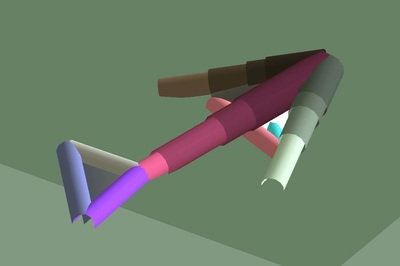
\includegraphics[height=5cm]{fig/arrow-hires1.jpg}
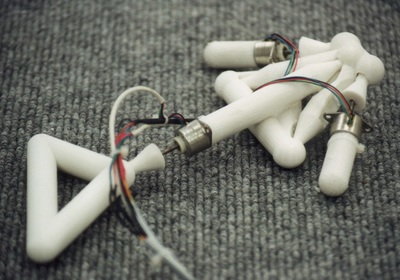
\includegraphics[height=5cm]{fig/arrow-hires2.jpg}
\caption{\label{fig:lipson}%
\textbf{Lipsonian AI.}
An evolved simulated robot (left) and its 3D printed equivalent (right) \cite{lipson2000automatic}.
}
\end{figure}

Although Sims, Ventrella, Lipson and Pollack, and many, many others \cite{ventrella1998designing,lichtensteiger1999evolving,ray2001aesthetically,bongard2003evolving,hornby2002creating,komosinski2001comparison,komosinski2003framsticks,hotz2004asymmetric,vaughan2004evolution,shim2006evolving,bongard2006resilient,chaumont2007evolving,bongard2010utility,auerbach2010evolving,auerbach2010dynamic,lehman2011evolving,hiller2012automatic,cheney2013unshackling,cheney2014electro,lessin2013open,auerbach2014environmental,cheney2015tight,brodbeck2015morphological,lessin2015soft,cellucci20171d,cheney2018scalable,rosser2019sim2real} used an Evolutionary Algorithm (EA),
% \cite{fogel1998evolutionary}),
evolutionary robotics is independent of the specific procedure used to automatically generate and test designs.
EAs happen to be particularly useful in this domain because, apart from being exceedingly simple and parallelizable (Algorithm~\ref{alg:evo}),
% The benefit of evolutionary algorithms is that 
few assumptions must be made about the robot \textit{a priori}.
The robot's material properties, building blocks, structure, shape, configuration, and controller can all be optimized together.
For 25 years, structural optimization proper---changing the number and placement of mechanical degrees of freedom (building blocks), not merely tuning the parameters of a predefined structure---had only been achieved through evolutionary design.



% \newpage
\section{Evolutionary Algorithms}

% There are however two important respects in which EAs differ from RL.
Evolutionary Algorithms \cite{fogel1998evolutionary,cliff1993explorations,floreano1996homing,harvey1997evolutionary,nolfi2000evolutionary} differ from ``gradient-based'' approaches to optimization in two important respects.
First, EAs require a population of agents (candidate designs) spread out on the fitness landscape,%
\footnote{%
A ``fitness landscape'' is a metaphorical terrain
used to conceptualize multidimensional design space in terms of more familiar notions of topographical space.
Design variants are mapped to coordinates on the horizontal axis (Fig.~\ref{fig:baldwin2d}) or plane (Fig.~\ref{fig:baldwin3d}).
The elevation of this landscape is fitness (higher is better).
Unlike a phase-space or field, which describes the tendency of state transitions in ontogeny, a fitness landscape describes changes in fitness due to changes in design.
There is no guarantee that mutations exist to move a design up a slope of fitness.
% The true shape of the fitness landscape is protean and unknown, but local gradients
% (a series of design revisions yielding progressively better fitness) 
% can sometimes be estimated under simplifying assumptions about the robot's 
% % body and environment (and their interactions),
% body and world, such as constraining the design to be a fixed structure that is parameterized and tunable but not addable/removable.%
} 
whereas learning occurs within a single agent.
Second, individuals in an evolving population are modified through random mutation, without any anticipated benefit.
Gradient-based learning algorithms, in contrast, predict the repercussions of design revisions before applying them;
they estimate the local topography (the gradients) of the fitness landscape around the current design,
so that revisions can be applied that are expected to improve the design (climb the gradient).
% simplifying conditions.
% more circumspectly.
Evolution has no such foresight.

% \vspace{1em}

\begin{algorithm}
\caption{\textbf{Evolution.}}\label{alg:evo}
% \vspace{-8pt}
% \noindent\rule{\textwidth}{0.5pt}
\begin{algorithmic}[1]
\State $\mathcal{P} \gets$ CreateRandomPopulation() 

\While{\textbf{not} TerminationCondition()}
\State EvaluatePopulation($\mathcal{P}$) \Comment{\small$n$ individuals evaluated at once on $n$ threads}
\State $\mathcal{S} \gets $ SelectParents($\mathcal{P}$)
\State $\mathcal{P} \gets $ RecombineAndMutate($\mathcal{S}$)  \Comment{\small appends or replaces $\mathcal{S}$ with mutants}

\EndWhile
\State \Return GetFittestIndividual($\mathcal{P}$) 
\end{algorithmic}
\end{algorithm}




% \newpage
\section{The March of Progress}


In 2019, \citet{pathak2019learning} demonstrated how a robot's 
ontogenetic structure and configuration
% physical structure and
% % neural
% configuration
% controller 
can be co-optimized using a gradient-based reinforcement learning (RL) algorithm, without evolution.
Instead of evolving a monolithic morphology, Pathak et al.~optimized a swarm of elemental agents---autonomous ``limbs''---that, in addition to actuating, could choose at every timestep to either attach to their nearest neighbor (forming an aggregate, symbiotic machine with a shared reward function) or detach, reconfigure, and test a new design.%
\footnote{%
Simply put,
attaching/detaching was in the ``action space'' of each limb \cite{sutton2018reinforcement}.
}
Thus structure was controlled by the same policy that coordinated 
% configuration.
behavior (configuration change).


Despite not using an Evolutionary Algorithm, this too is evolutionary robotics.
Indeed, the line between RL and EAs 
is becoming so thin, the two are almost indistinguishable.
There are EAs that act more like a single agent learning than a population evolving \cite{salimans2017evolution}.
% multi-agent systems
And with the rise of massively parallel computer architectures,
increasing interest in RL is coming to bear on population-based methods that can fill up those parallel threads with multiple learners  \cite{jaderberg2019human}.
% Ultimately, evolution and learning operate on different timescales but they are at root the same algorithm: Generate and Test \cite{dennett1975law,Dennett95}.
% But if Evolutionary Robotics is eventually rebranded as Deep Development, so be it.
What's clear is that Pathak's virtual robots evolved in the colloquial sense of the word.
If we compared the structures assembled by randomly generated limbs to those assembled by fully trained limbs, and sampled some results along the way, we would get something like Rudolph Zallinger's iconic ``March of Progress'' from Dryopithecus to Modern Man, that inevitable stock image of evolution.
There is no march of progress for non-evolved robots because the design is held fixed during training.



However, there hasn't been much of a march of progress for evolved robots either.
Despite vast increases in computational power since 1994
and major advances in additive manufacturing after 2000,
evolutionary robotics has floundered in a sea of Sims-like virtual creatures (Fig.~\ref{fig:sims}) and Lipsonian machines (Fig.~\ref{fig:lipson}).
Apart from the work documented in this thesis,
there have only been three examples  \cite{hiller2012automatic,brodbeck2015morphological,cellucci20171d} of evolved robots published since \citet{lipson2000automatic}.
% primordial crawlers.
% (This thesis contributes a few more.)
Even in silico,
free from most real world constraints,
scant progress has been made scaling the complexity and competence
% , and usefulness 
of virtual robots \cite{cheney2016difficulty} (Fig.~\ref{fig:sims}).
% and their 3D printed equivalents
% \cite{cheney2016difficulty}.


\begin{figure}
\centering
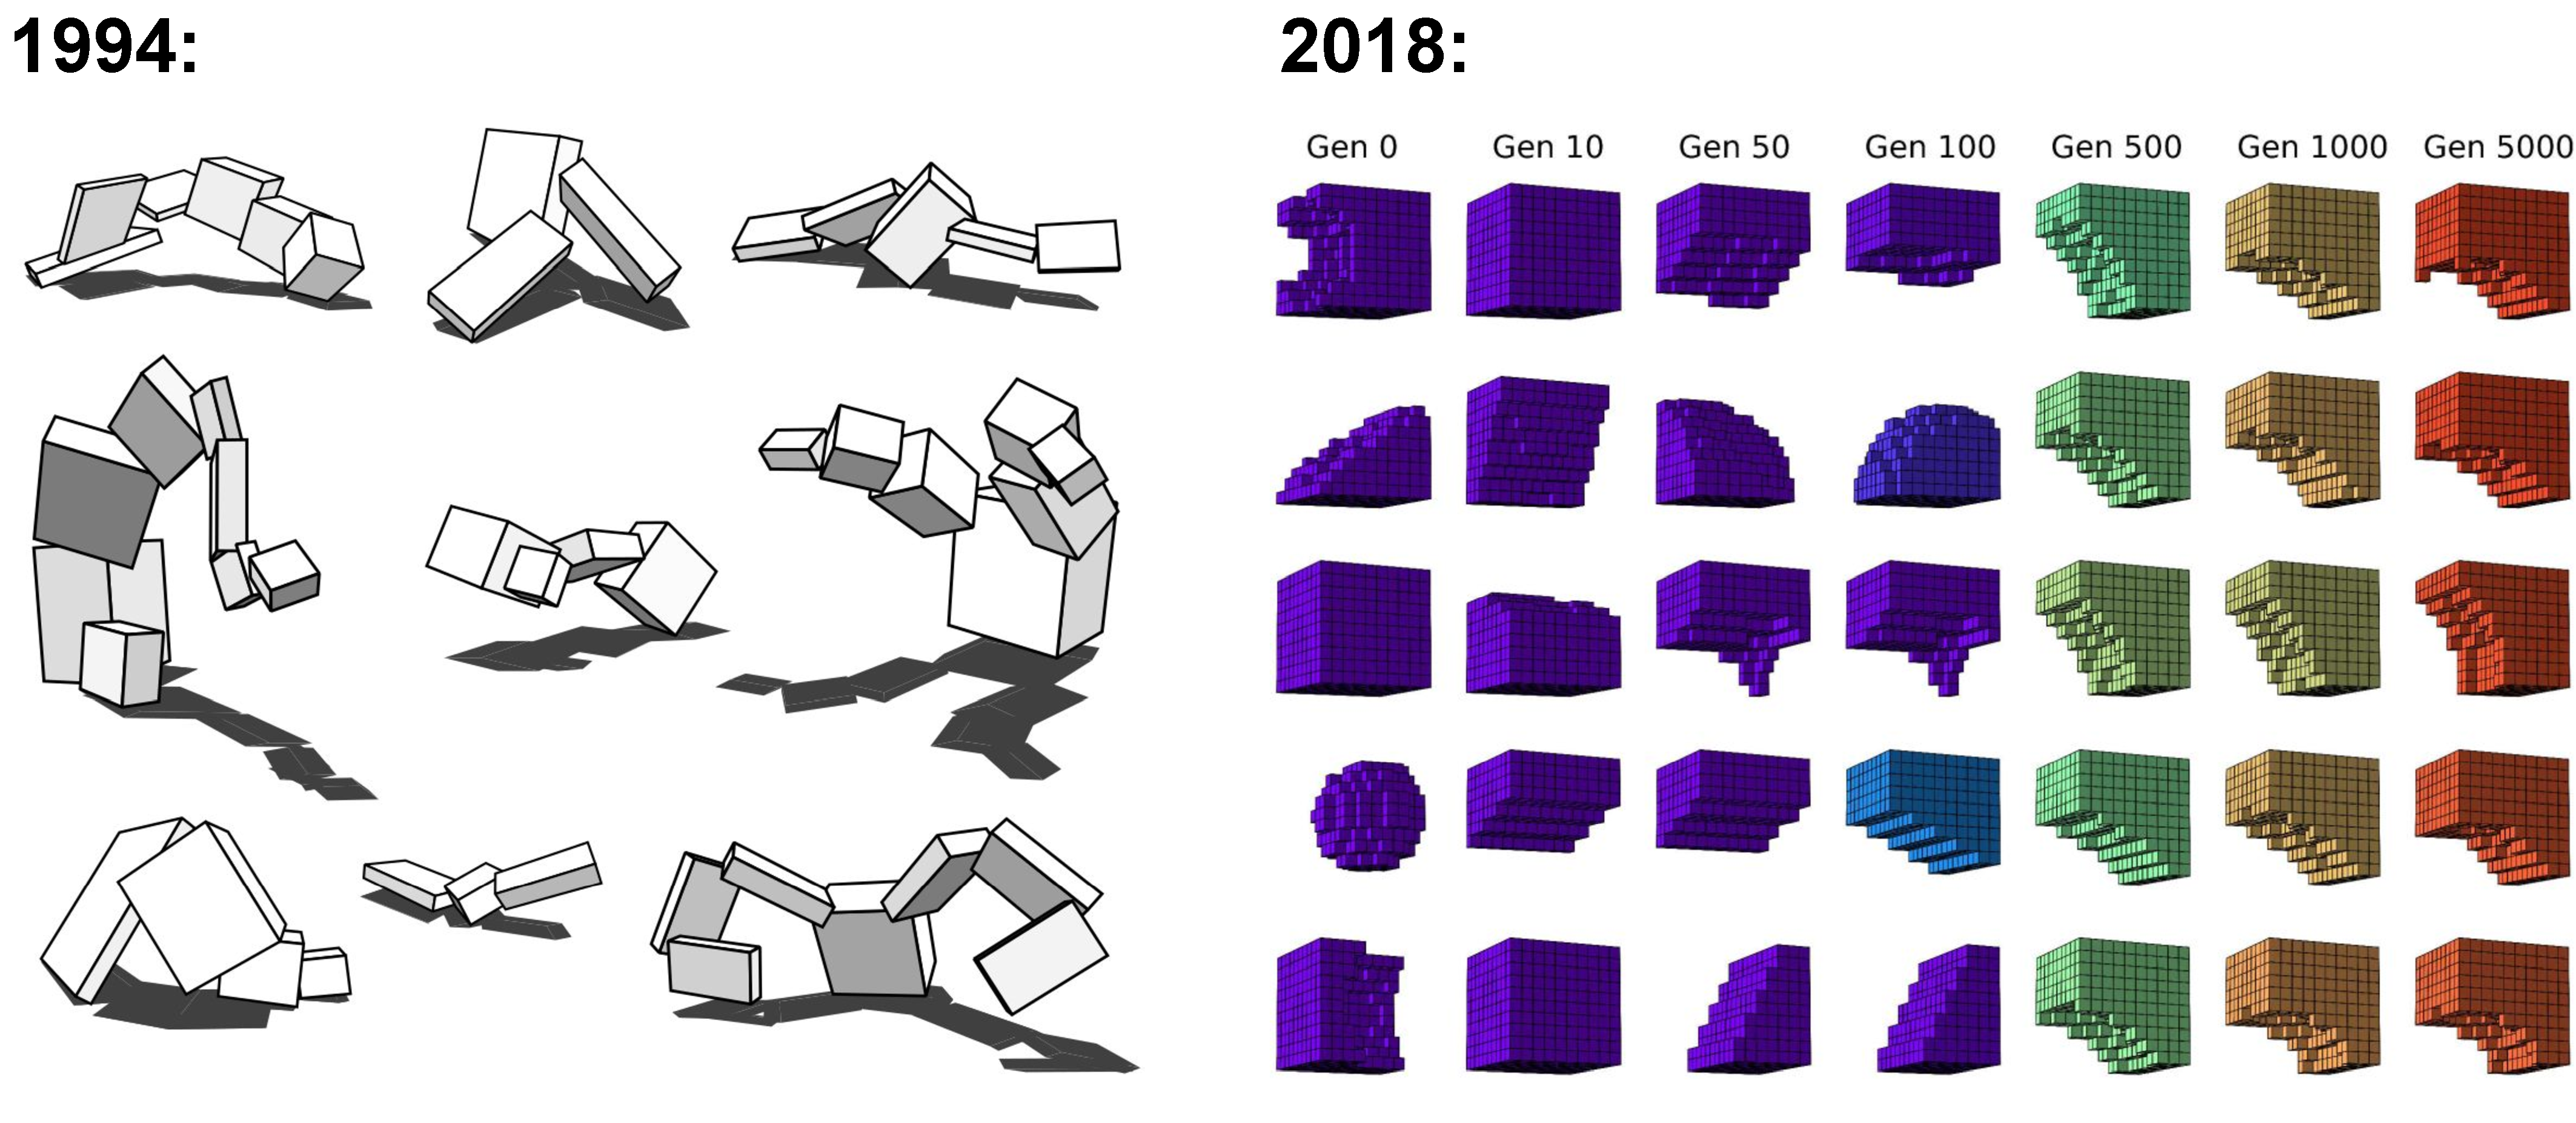
\includegraphics[width=\linewidth]{fig/virtualevorobo.pdf}
\caption{\label{fig:sims}%
The first evolved simulated robots (Sims, \cite{sims1994evolving}), and the state of the art (Cheney et al., \cite{cheney2018scalable}).
}
\end{figure}



% Optimizing robot hardware is tricky.
% Vanishingly small changes to a physical structure can cripple its behavior.
% If the ability to change is a necessary precondition of adaptive behavior, it is not sufficient.
% Some changes are beneficial; other changes are deleterious.
% Sometimes the best thing to do is remain the same.
% Protean machines must therefore be optimized to bring about appropriate morphological change in response to environmental conditions.
% Many forms of optimization exist.
% A natural choice is evolution.

% Learning algorithms presupposed a structure and only adjust its parameters. 
% parametric changes to a fixed structure
% blind, unconscious

% The benefit of evolutionary design is that few assumptions must be made about the robot a priori.
% The robot's material properties, structure, shape, and control policy can all be optimized together.
% Despite this potential, most experiments begin by presupposing an overwhelmingly static robot---with fixed mechanical structure, material properties, and resting shape---and expose only its control system to evolutionary improvement \cite{nolfi2000evolutionary}.
% These experiments thus evolve controllers, but not robots.



\section{The Evolvability of Robots}


One reason that evolving robots 
% at scale
has proven so challenging is the very fact that robots are embodied and situated.
Local structural revisions, such as adding a fifth rotor to a functioning quadcopter, tend to have global behavioral repercussions.
Thus, it is usually challenging to find a series of small adjustments that result in increasingly better design. 
This property makes physical artifacts much more difficult to optimize than disembodied systems such as deep neural networks, which tend to preserve their behavior in the face of sweeping global revisions.\footnote{%
The most common method for training artificial neural nets is backpropagation of error, which
estimates the gradient with respect to each weight of the network.
Iterating backward, one layer at a time, error is propagated by chain-rule to upstream weights, which are adjusted in proportion to their respective gradient.
Depending on the size of the network, thousands or millions of parameters are all perturbed at once.%
}

Certain aspects of robot behavior are generated by the precise orchestration of its parts.
When these parts change, such as by the lengthening of a single leg, the control policy could be rendered more or less obsolete, and either a small software patch or larger update will be necessary to regain control over the new hardware.

Other aspects of behavior are generated by virtue of embodiment and the laws of physics alone, such as rolling down a declined plane, and the swing phase of human walking.
From the controller's perspective, such behaviors, or aspects thereof, are passive: the body and world provide them ``for free''.
The control system need not spend any of its valuable resources orchestrating this behavior from scratch; instead, it may exploit these passive dynamics, gently guiding them when necessary, to render useful work.
However, if control is predicated on certain body-world interactions occurring automatically, then even sight changes to the body can result in catastrophic failure.
In the worst case, the controller could be considered ``totaled'': it's cheaper to evolve a totally new controller or robot than to repair the existing system.

Thus, much work has attempted to reduce the behavioral repercussions of morphological change \cite{cheney2018scalable}.
A natural way
to reduce the behavioral impact of a mutation 
is to spread that impact across a period of time: development.



\section{The Evolution of Development}


In a population of evolving but non-developmental robots, mutations can only change the physical layout by discrete steps, from parent to child.
This is because the design of a non-developmental robot cannot change during its lifetime.
The morphological and thus behavioral impacts of such mutations kick-in immediately, at $t=0$.
Introducing development allows mutations to manifest slowly during the lifetime of a robot, or at the very end of the lifetime, which enables arbitrarily small design modifications.

Of course there are other ways to reduce the behavioral impact of mutations.
For one, we could simply restrict the magnitude of morphological mutations to be vanishingly small.
This might very well be sufficient given enough time, and if the fitness landscape is smooth enough to ensure that a sequence of tiny steps will progressively increase fitness.
However, the search space of possible robot designs tends not to be smooth in realistic settings; rather than hills and gentle slopes, the landscape is typically full of cliffs and harsh spikes. 

Some great designs, we may suppose, are only of value when perfect or nearly so; changing them by even a single bit is all but certain to entirely break their functionality.
In other words, there is no gradient---no sequence of mutations---leading toward these great designs.
In such a space, a near miss is as good as a mile, and evolution can be no better than random search.
However, as Hinton and Nowlan \cite{hinton1987learning} so neatly demonstrated: development can (under the right conditions) smooth the search space that evolution operates in, thereby creating a gradient toward increasingly better mutations (Fig.~\ref{fig:baldwin2d}).


\begin{figure}[t]
\centering
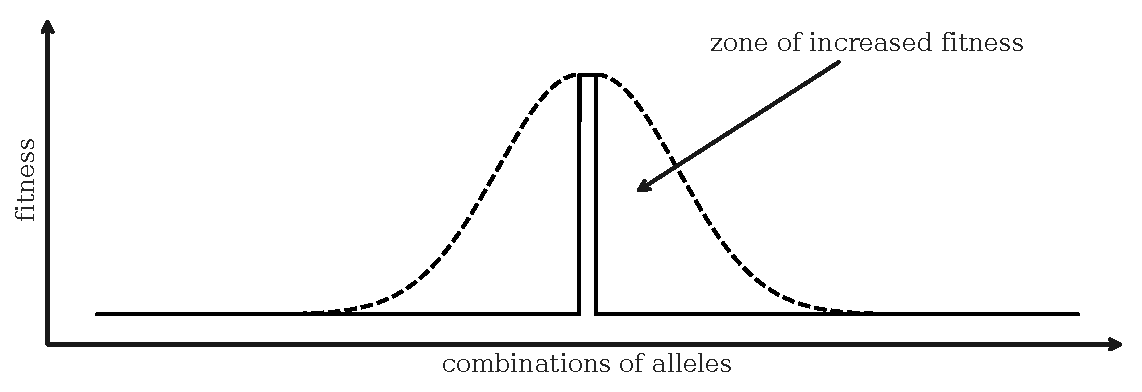
\includegraphics[width=\linewidth]{fig/Baldwin2D}
\caption{\label{fig:baldwin2d}\textbf{The Baldwin Effect.} Hinton and Nowlan \cite{hinton1987learning} considered the evolution of a bitstring that is only of value when perfectly matching a predefined target string. 
The search space of possible combinations of alleles (bit values) therefore has a single spike of high fitness with no slope leading to the summit (solid black line).
``The good [string] is like a needle in a haystack.''
Here's where development, through the so-called ``Baldwin effect'', can potential guide evolution:
Suppose that the ``lifetime'' of each bitstring is lengthened from a single point to a period of time in which a portion of the string can change. 
Then there is a chance that some string in flux, eventually, flips the right bits and stumbles upon the good static string during its life.
If evolution controls which portions of the string are flippable and which are non-flippable (i.e.~genetically determined),
and the later are all correctly specified,
then the speed at which such individuals tend to hit the target will be proportional to the number of non-flippable bits.
Finally, it is reasonable to assume that the faster an individual discovers the good design during its lifetime, the more fitness it accrues.
Taken together, this has the effect of creating a gradient of increasing fitness (dotted black line), leading up to the correct specification, that natural selection can climb by incrementally hardcoding more correct bits in the genotype.
``It is like searching for a needle in a haystack when someone tells you when you are getting close.''
(Redrawn from \cite{hinton1987learning}.)
}
\end{figure}


This process, known as the Baldwin effect \cite{baldwin1896new,simpson1953baldwin,dennett2003baldwin}, is possible because development sweeps over several traits in a single agent, and sometimes exposes promising static traits along the way.
This can create a new gradient in the evolutionary search space, rewarding descendants that more rapidly manifest the good trait during their lifetimes (and retain it through the remainder of their lifetime).
Following the gradient requires a series of mutations that incrementally reduce development such that the good trait becomes ``locked-in'' in more morphologically-static descendants \cite{waddington1942canalization}.
Development is thus a ladder that, like Wittgenstein's, can be thrown away once it has been climbed.
However this is only possible if such mutations exist.


When a behavioral change manifests late in the lifetime of a developing robot, it might discover a promising static design at the end of its life.
The sequence of mutations required to prepone or ``earlify'' this trait such that it arises increasingly earlier in the lifetimes of descendants, might be hard to find or might not exist at all.
Symmetrically, if a promising static design is discovered early in the lifetime of an robot, but the robot develops out of it, the hypothetical series of mutations that prolong this behavior may be 
% a chimera. 
illusory or impossible to execute without completely disrupting behavior.
Indeed, one of the first experiments to explore the interaction between evolution and (neurological) development in controllers onboard real robots \cite{floreano1996plastic}, found that such mutations are unlikely to exist if agents exploit developmental change for behavior.

\begin{figure}
\centering
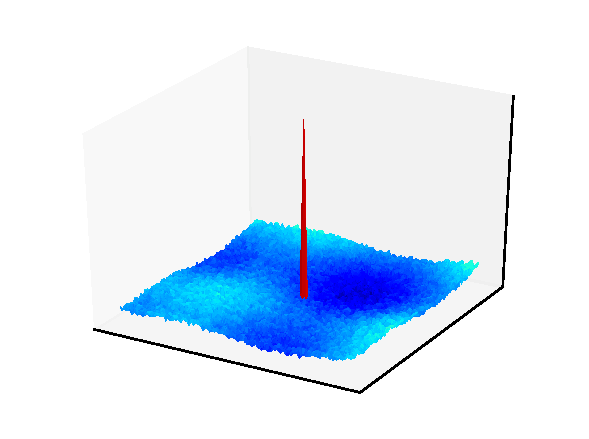
\includegraphics[trim={40pt 20pt 30pt 25pt},clip,width=0.49\linewidth]{fig/baldwin_rugged.pdf}
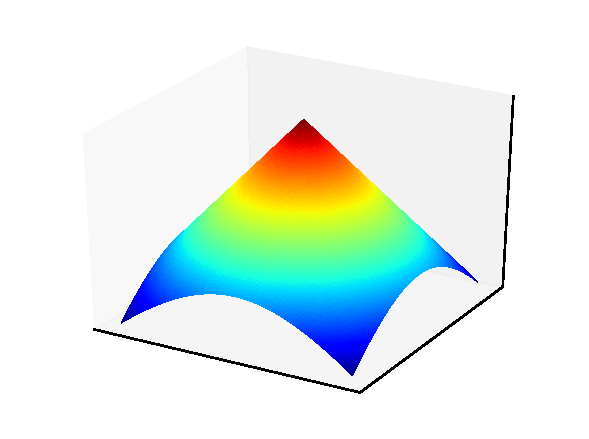
\includegraphics[trim={40pt 20pt 30pt 25pt},clip,width=0.49\linewidth]{fig/baldwin_smooth.pdf}
\caption{\label{fig:baldwin3d}\textbf{Two sides of the same space.} 
In each plot, points on the horizontal axes directly map onto a 2D continuous design space.
For example, $x$ could encode the initial elastic modulus of a bipedal robot's two limbs, and $y$ might then indicate their initial placement along the circumference of its spherical trunk.
The vertical axis is fitness.
On the left, we have a highly-fit genotype (red spike) among a sea of designs with much lower fitness (blue waves).
The red design might be an upright bipedal walker with the appropriate elasticity,
while the blue designs perhaps can only scoot, tumble, or row themselves forward (if they can move at all).
On the right: the aftermath of the Baldwin effect.
Developmental plasticity alters the space by introducing a gradient: 
Proximity to the great design determines the speed and reliability with which it may be expressed during development, and thus determines (expected) fitness.
}
\end{figure}

When picturing Hinton and Nolwan's idealization as a single column of high fitness in the middle of an abstract 1D design space (Fig.~\ref{fig:baldwin2d}), it can be difficult to imagine how evolution moves through a real, multidimensional search space. 
So at the risk of being redundant, 
I've included a second depiction of the Baldwin effect (Fig.~\ref{fig:baldwin3d}) in which the vertical axis is again fitness, but in which the horizontal axes directly map onto continuous parameters of the design.
Development unfolds on a line in this space, with the vast majority of possible trajectories missing the good trait combination.%
\footnote{%
There are typically many such (potentially Baldwinifiable) local optima, and so there is also evolution: a population spread out on the landscape, not just a single developmental robot.%
} 
Let's call the good one ($x^*,y^*$).
Evolution discretely samples the space by setting the initial conditions ($x_0,y_0$) and how development may unfold across the landscape (curvature and length of the line) in time (acceleration along the curve) until death ($x_{\tau},y_{\tau}$).
Once found, successful developmental trajectories can become canalized by evolution such that the good trait combo becomes increasingly likely in future descendants.
In the limit the line of development shrinks until $(x_0,y_0) = (x_{\tau},y_{\tau}) = (x^*,y^*)$.

% Note that it is also possible for a continuum of highly-fit variations on a design to exist on a manifold that is isolated from the surrounding search space.



\section{Evolved Development in Robots}


\citet{hinton1987learning}, and the cascade of subsequent computational/analytical studies to investigate this interplay of evolution and development,
considered either abstract phenotypes \cite{belew1989evolution,ackley1991interactions,nolfi1994learning,french1994genes,mayley1996landscapes,ancel1999quantitative,ancel2000undermining,sendhoff1999model,suzuki2004interactions,downing2004development,santos2015phenotypic,fernando2018meta,todd2020interaction}
or control systems onboard morphologically-static hardware \cite{floreano1996plastic,husbands1998better}.
Evolution and development could not modify body plans because, without exception, the body plan (if it existed) was fixed.

Several computational but embodied models of prenatal development have been forwarded
\cite{dellaert1994toward,dellaert1996developmental,Eggenberger97,Bongard01,miller2004evolving,basanta2008evolution,doursat2009organically,doursat2014growing,joachimczak2016artificial}.
However, because development occurred prior to the evaluation period,
as a kind of artificial embryology,
the behavioral impact of a mutation 
% in these studies 
still kicked-in at ``birth'' ($t=0$), and so the Baldwin effect could not occur.


Prior to the work documented in this thesis, there were only three cases reported in the literature in which a simulated robot's body was allowed to change while it was behaving. 
In the first two cases \cite{ventrella1998designing,komosinski2003framsticks}, it was not clear whether this ontogenetic morphological change influenced the evolution of behavior in any way. 
Later, Bongard \cite{bongard2011morphological} demonstrated how such change could lead to a form of self-scaffolding that smoothed the fitness landscape,
not unlike the Baldwin effect.
% and thus made optimization much easier.
But the Baldwin effect did not occur, because it could not occur.

Bongard's experiments began on familiar ground.
Populations of neural controllers were evolved to
steer (the configuration of) a simulated quadruped/hexapod so that it moved toward a simulated light source.
But this robot had a trick up it's four (or six) sleeves.
The robot was, for most of its evolutionary history, deployed with an anguilliform body plan---an eel with an actuated spine.
As the initially legless robot behaved (i.e.~during configuration changes),
limbs were slowly extruded from its trunk,
like a quartet (or sextet) of trombones descending in pitch.
As the limbs lengthened, they dipped their resting angle about the shoulder joint, transitioning the robot from a prone to upright stance, during development.

Early in evolution, limb growth occurred over the robot's entire evaluation period.
In a series of four evolutionary stages,
the rate of extrusion was incrementally increased
such that the final, upright legged body plan was realized increasingly earlier in developmental time, and held fixed for the remainder of the robot's lifetime.
In the final stage of evolution,
the robot was deployed with its final shape from the very beginning of its behavior; development had been completely canalized.
% transitioned once a controller was found that was capable of phototaxis under the prescribed developmental schedule

Thus, by the end of evolution, these robots were identical to a control treatment but for a single isolated difference: one group had ancestors that developed, and the other had ancestors which did not develop.
However, this clean experimental design came at a cost: the robot's initial shape, and the way in which its shape developed, were both manually fixed \textit{a priori}. 
Thus evolution could not modify morphological development, indeed, it could not modify morphology at all.\footnote{%
The trombone trick used by \citet{bongard2011morphological} was also employed by a 
% carbon fiber 
later robot to automatically adjust leg length in situ for different supply voltages \cite{nygaard2018real} and terrain
\cite{nygaard2020environmental}.
However, leg length did not vary during behavior (locomotion), so the Baldwin effect could not occur.
}



% \newpage
\section{Resilient Machines}


\begin{changemargin}{4em}{4em} 

\vspace{1em}

    \textit{Only variety can destroy variety.} \\[4pt]
    \hspace*{16.5em} ---W.~Ross Ashby (1956)
    
\vspace{1em}
    
    
\end{changemargin}


\noindent
It is often the case that an artificial system may be trained to achieve high fitness in one environment, but fail spectacularly under even the slightest perturbations \cite{athalye2018synthesizing,carlson2005ugvs}.
By temporarily permitting shape to vary during training, the final, manually-canalized robot from  Bongard's experiment \cite{bongard2011morphological}
% (and others, such as   \citet{vaughan2004evolution})
% also showed how temporarily permitting a few design elements to vary during training can 
exhibited increased robustness in novel environmental conditions (random external perturbations).
% inborn
Shape change thus acted as a form of regularization: 
the robot had to maintain phototaxis while changing its body.
This increased breadth of sensor-motor contingencies prevented the robot from overfitting its controller (of configuration) to the idiosyncrasies of a small sample of circumstances \cite{jakobi1995noise}.
% exposure
The upshot was robustness by virtue of a good static structure.
% Like a bridge that dissipates rather than amplifies vibrations
% it is less likely to crumble under harmonic oscillations
% \cite{cheney2014automated}.
% But this form of robustness can only stretch so far ``out of sample'', outside the set of circumstances experienced by the system during training.
% The fitness landscapes that evolution climbs, and development sometimes smooths, tend not to remain static in realistic settings:

% Environmental conditions are protean and unpredictable.
% It is therefore advantageous to leave some aspects of design plastic rather than hardcoding them as fixed features.
However, for a system to remain viable as its environment varies, the system must also be able to vary itself.
Only variety can destroy variety, as Ashby put it.
% A plant constrained to grow along a fixed path will, for instance, capture less light than a plant that varies its growth toward sunlight.
Thermostats, centrifugal governors, and Ashby's Homeostat\footnote{%
The homeostat was built by Ashby in the late 1940s using surplus military equipment.
It consisted of four identical electrically-coupled units.
Each unit sent its output to, and received an input from each of the other three.
A pivoted magnet sat atop each unit.
DC output was proportional to the angular deviation of the unit's magnet from its central position.
The magnet's deviation was in turn a function of input, internal circuitry, and 
% four 
adjustable parameters supplied by stepping switches.
When current exceeded a certain value, the switches were energized, moving the parameters to new values.
% (A maximal switching frequency was set by a device that locally interrupted power at regular intervals.)
The field (defined in section \ref{sec:ontology}) of the Homeostat's four variables (magnet positions) had only one state of equilibrium (centered), which was either stable or unstable.
When the magnet's position was perturbed externally by mechanical force, the system would cycle through switch settings according to a random number table until it found a stable field and reached equilibrium, where it would actively resist subsequent external perturbations.
}
are examples of such systems---regulators---with the ``requisite variety'' to
% destroy 
absorb and eliminate
variety in the system being regulated.
The field of each of these regulators is ``ultrastable'', as Ashby would say, tending all the time towards stabilization and
physiologic constancy.
However, these regulators are controllers (Fig.~\ref{fig:policy}), not robots.\footnote{Any system that cannot move through the world has at best a questionable claim to be a robot.}
% Six decades after the Homeostat, 
% Six centuries after the invention of the thermostat, two centuries after the invention of the governor
% across the pond, at Cornell University, 

In 2006,
\citet{bongard2006resilient} reported a ``resilient machine'' that, through continuous self-modeling,
could vary its behavior to compensate for structural loss due to damage.
% \footnote{%
% Whereas thermostats, governors and homeostats are robust---their field is stable---this robot was resilient: able to change the field for a new environment.
% Rather than cycle through all possible behaviors randomly (which is inefficient), or learn through reinforcement in the real world (which is risky),
% the robot internally rehearsed actions, discarding those that were unsuccessful or dangerous, before attempting them in reality.
% It could, as Karl Popper once put it, let its hypotheses die in its stead (\cite{popper1972objective}, p.~122).
% % ``Scientists try to eliminate their false theories,
% % they try to let them die in their stead.
% % The believer---whether animal or man---perishes with his false beliefs.'' Karl Popper, 1972 (p.~122, \cite{popper1972objective})
% }
The details are not 
important for the story I have chosen to tell about increasingly protean machines,
beyond noting the relationship between regulators and models, which was made clear by \citet{conant1970every}:
\begin{quote}
\small
\dots success in regulation implies that a sufficiently similar model must have been built, whether it was done explicitly, or simply developed as the regulator was improved.
\end{quote}
In this case, explicit body schema were built from the ground up, in silico, through sensorimotor experiment in the physical robot.
Because the robot modeled its structure, rather than just its behavior, it could absorb variation in both.
Later, \citet{cully2015robots} demonstrated how a robot could in some cases do this much faster.
% These two robots are more autonomous than conventional robots which require repair from a human operator.
However in both approaches, the mechanical details of the robot (structure/material/shape) were presented to the control system as a \textit{fait accompli},
limiting the depth of insult 
% such machines can destroy.
from which such machines can recover.


These two studies were at the bleeding edge of robotics and will undoubtedly be refined with additional R\&D.
% They will likely find themselves onboard future robot expedition teams within the depths of Europa's subterranean sea.
% That these particular machines could barely cope with even the slightest tribological changes in terrain (\citet{bongard2006resilient} needed a pane of plexiglass between their robot and the carpet to enable locomotion) can be resolved by better static hardware.
In the meantime, they seem to have spelled out the limitations of clever software trapped inside non-protean machines.
Such
behaviorally-plastic yet morphologically-static robots can recover masterfully from certain shallow insults, such as the
loss of a single leg to injury.
% to coordinate their fixed parts the currently has.
But they do not have the requisite variety to recover from deeper mechanical damage, such as the removal of all limbs or being chopped into a hundred little pieces.

It's not just that they can't re-generate structure, motors or sensors.
It's that they can't generate these things in the first place.
Their ability to perceive the environment, and act against it, 
is constrained within a fixed set of perceptual categories and action alternatives, rather than open-ended.
% Prespecified perceptual categories and action alternatives 
This shackles the robot's epistemic autonomy \cite{cariani1993evolve}:
the robot's overall capacity for 
knowledge 
% adaptive behavior
and cognitive success beyond what
the designer predicted to be relevant for the problem at hand.
% before the robot was out of reach.

% percepts and action alternatives
% have the freedom to adapt within a set of percept
% and action categories, but they do not have the freedom to modify those categories.

% Ashby accepted these constraints in building his framework on top of a core
% assumption that the state of a machine could be boiled down to a fixed set of variables, each of which could be represented by a pointer on a dial.
% Most of the dials will be pointing to zero, as
% Ashby (\cite{ashby1952design}, p.~14)
% noted:
% \begin{quote}
%     \small
%     The absence of an entity can always be converted to a reading on a scale simply by considering the entity to be present but in
%     zero degree.
% \end{quote}
% Ashby admitted that there are, in fact, infinitely many such variables (ibid, p.~15):
% \begin{quote}
%     \small
%     \dots\textit{every real `machine' embodies no less than an infinite set of variables}, all but a few of which must out of necessity be ignored.
% \end{quote}
% The problem was to find regulators capable of keeping the ``essential variables'' within physiological limits.
% Disturbances to a machine's essential variables could have either small effects or induce a large change of step-function form on the parameters (Fig.~\ref{fig:ashbyStepMech}).
% A part could be lost in an instant: dials associated with that part are zeroed.
% A part could also be slowly generated: dials previously set to zero are gradually turned up.
% But this stretches the metaphor too far, I think, to be useful.

% This change could be represented by an infinite set of variables, true, but some infinities are bigger than others.
% For instance, there are infinitely many ways to place a single limb on a given torso, let alone four limbs, or fractals of branching limbs and fingers.
% There are infinitely many ways to shape a finger, for that matter.

% So we are left with an Avogadro's number of ``essential variables''

% To Ashby, the field of a machine depends on its mechanical structure.
% When that structure breaks, the field changes.
% Some fields are lead to equilibrium that is stable, others do not, so the knobs are turned by a regulator until this is rectified or else the machine dies.



% \newpage
\section{A Protean Machine?}

\begin{changemargin}{4em}{4em} 

\vspace{1em}

\textit{And so it was that two very tired young men trailed a microphone down into Baker Street from the upstairs window, and picked up the random noise of dawn traffic in the street. 
I was leaning out of the window, while Gordon studied the cell. 
``It's growing an ear'', he said solemnly} (ipsissima verba). \\[1em]
\hspace*{16.5em} ---Stafford Beer (2001)

\vspace{1em}

\end{changemargin}



\noindent
In 1956, on Baker Street in the heart of London,
% (or '57, the details are a bit hazy)
Gordon Pask and Stafford Beer grew an electrochemical ear.\footnote{%
The basic electrochemical system had been developed earlier in collaboration with A.~Addison,
a member of Heinz von Foerster's laboratory at the University of Illinois
(\cite{pask1961approach}, p.~107).
}



\begin{figure}
    \centering
    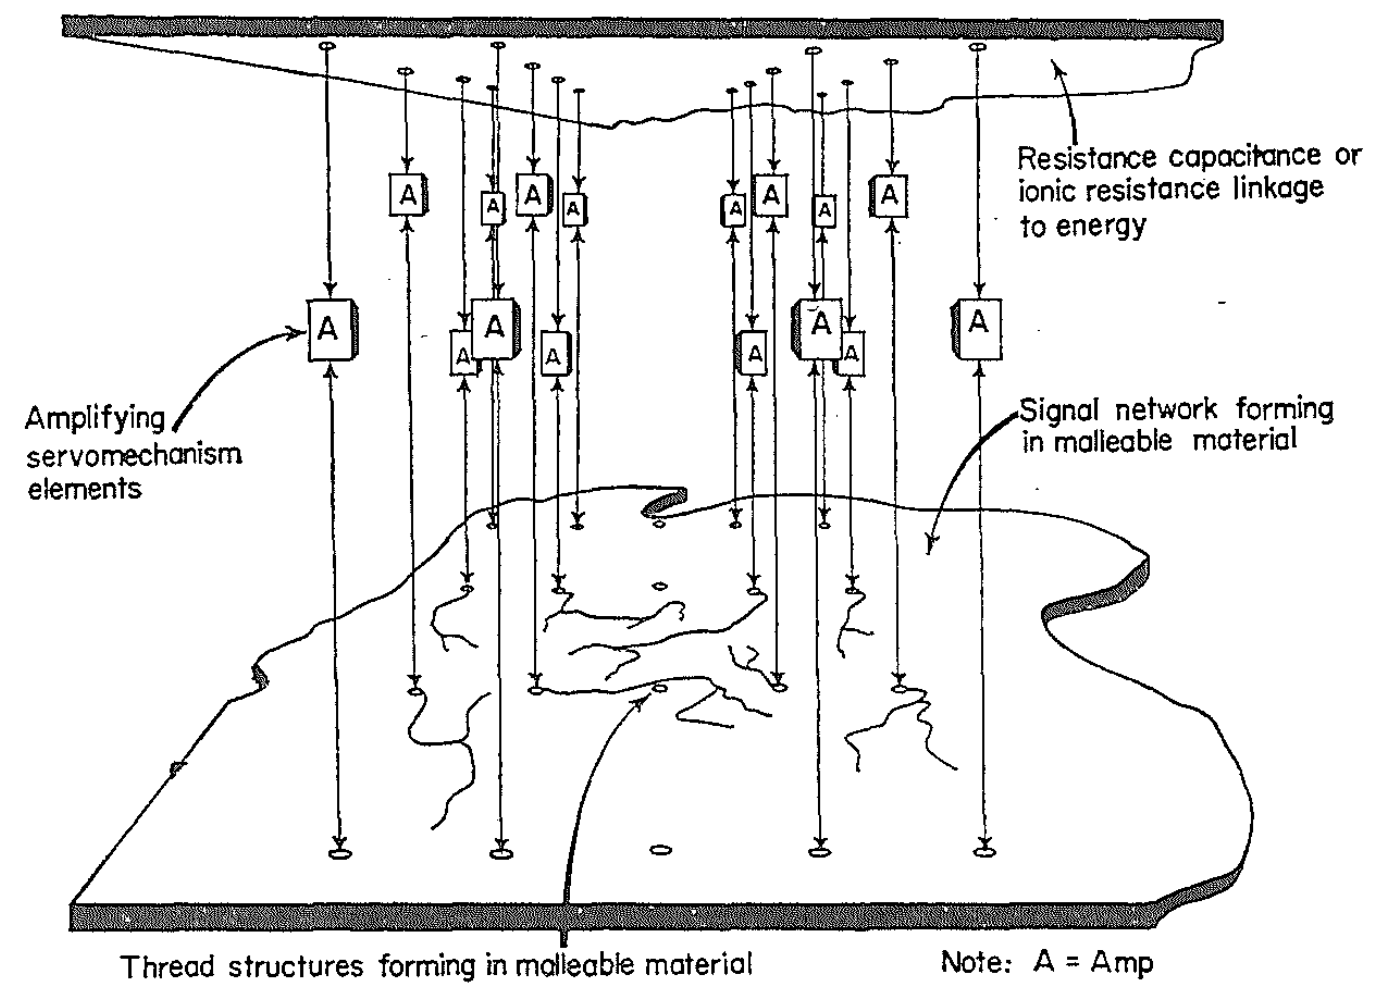
\includegraphics[width=0.7\linewidth]{fig/pask.png}
    \captionof{figure}{%
    \label{fig:ear}
    Electricity flows through an aqueous solution of iron salts, depositing low resistance metallic threads and influencing the subsequent flow of the current and metal
    (\citet{pask1960natural}).
    }
\end{figure}
\begin{figure}
    \centering
    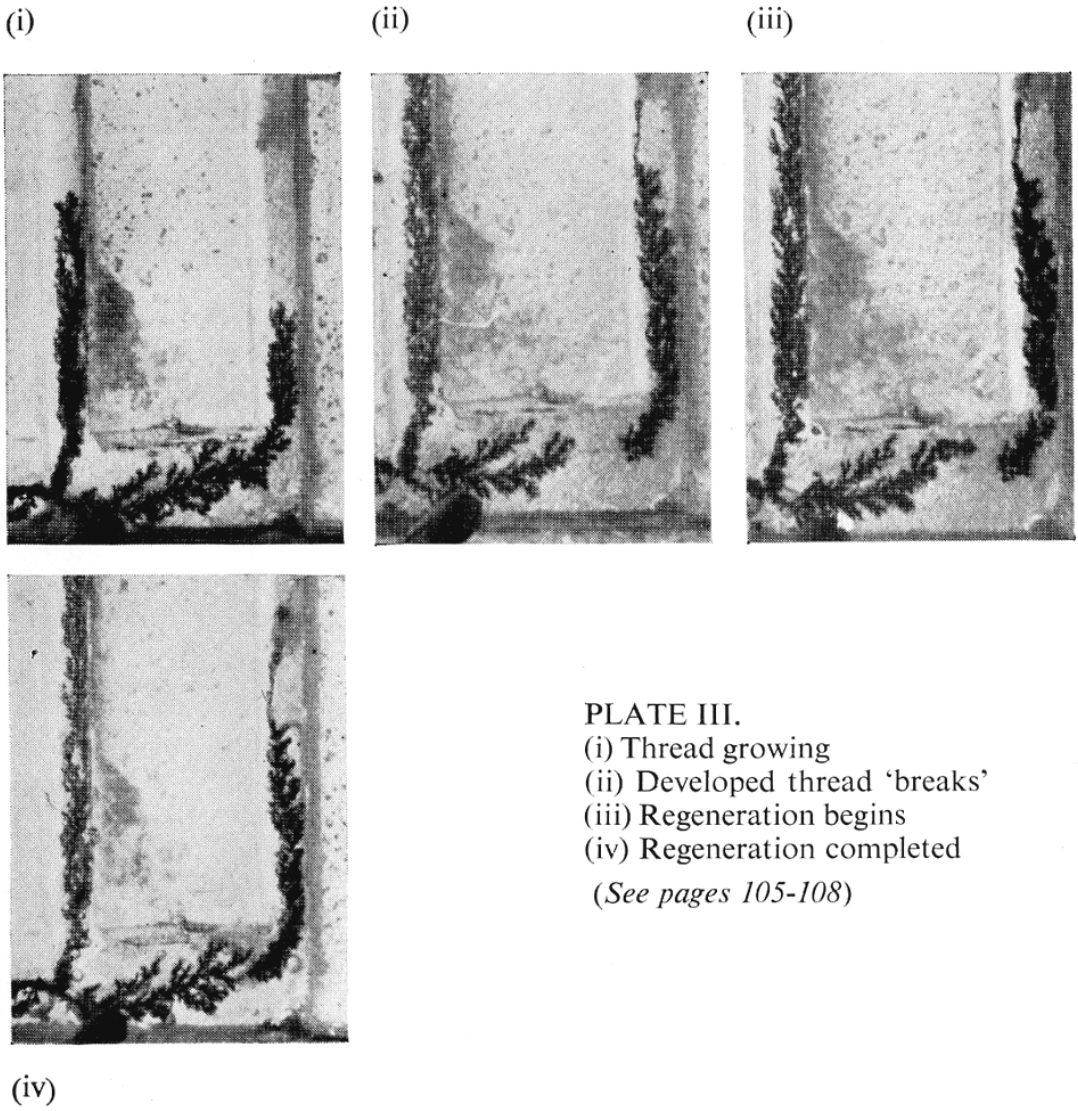
\includegraphics[width=0.65\linewidth]{fig/threads.png}
    \captionof{figure}{%
    \label{fig:threads}
    Dendritic threads of metal grow toward an electrode in iron-sulfate solution (\citet{pask1961approach}).
    }
\end{figure}



% recent perspectives:
% \cite{bird2008gordon} 
% \cite{pickering2002cybernetics}
% \cite{cariani1993evolve}  

% \cite{pask1961approach} details of thread growth and plate III
% \cite{pask1958physical,pask1960natural}: reported the ear here

% grow it's own ``relevance criteria''.
% tendrils, filaments, threads, trees, dendritic 
% when a decision is favored more current is allowed to pass.
% protean machine: whose boundaries are endlessly changing


% \cite{pask1961approach}:
Platinum wire electrodes were immersed in a shallow acrylic dish containing an
% moderately-conductive 
acidic 
aqueous metal-salt
% (ferrous sulphate)
solution
% and connected to a current-limited electrical source 
\cite{pask1958physical}
(Fig.~\ref{fig:ear}).
The flow of electricity through the solution caused the deposition of metal
on the floor of the dish
% and this deposit grows 
along lines of maximum current
% like a tree in the direction of each electrode 
(Fig.~\ref{fig:threads}).
% The resulting structure was functional
Metal deposits in effect extended the electrodes, generating circuits ab initio, 
instead of using components with their own well-defined forms and functions.
In this electrochemical soup,
there was only raw material: metal ions. 

As metallic 
% dendrites or 
threads were being built out of ions on relatively negative electrodes,
the acid worked to dissolve the threads back into ions.
Threads that kept pace with the acid back reaction, drew more current down them 
due to their very low resistance (relative to the solution) and were thus
% current will tend to flow down them, 
reinforced and extended with additional metal.
Growth was not linear, however.
Each thread was fringed 
% on all sides 
by short thin tendrils that extended into the solution in all directions, testing the waters as it were, before retracting back toward the main branch in perpetual dis/integration.
Under a constant input set of voltages,
threads
competed for current, grew and dissolved, broke and regenerated, bifurcated and sometimes combined before settling into
a dynamically stable network with asymmetrical structure and robustness.
% whose edges continued to ebb and flow.

The electrochemical assemblage also displayed a kind of memory.
When the input set of voltages were held constant, a big dense metallic tree grew steadily until it reached a stable structure.
If the input set was then changed, the tree slowly
shifted and
restructured itself.
If the input was then set back to the original distribution,
the tree regenerated the initial structure, but this time stability was achieved much more quickly.
This was because dissolution was gradual and 
residual particles helped subsequent threads grow back rapidly along the same lines.
The longer a tree had been stably growing, the slower it disintegrated when the input set of voltages changed, and the quicker it returned to its original structure when the inputs were reset.
That is, the robustness of the tree was determined by the conditioning time:
reinforcement learning was possible.

A sensor electrode was dipped into the solution.
The generated waveform of the electrical output could be conditioned by rewarding thread networks with an increase in current supply, which released an influx of free metal ions---the building blocks of threads.
As a result, certain types of structures were allowed to survive and grow while those that did not act appropriately could be
starved of ions and tended to die off. 
Pask noted that, regardless of how the electrodes where configured, the system would tend to develop a thread structure that lead to current flowing in such a way that it was rewarded further.
Keep in mind, this reward is simply an increased capacity for growth---there is no specification of what form the growth should take. 

Thread networks could be steered and selected to become sensitive to a wide variety of stimuli impinging on their structure.
Electrical output was noticeably affected by all sorts of variables, including, but not limited to: temperature, pH, magnetic fields, and vibrations.
So Beer and Pask took a microphone, 
hung it out of a window on Baker Street
and picked up noise from the street.
The electrochemical soup started to vibrate, and with reward, started to form a function in response to audio signals.
% new sensor modality

The device was later grown to recognize specific frequencies, as from a buzzer.
Whenever a buzzer was sounded,
if the electrical frequency of the buzzer was partially replicated at the sensor electrode, 
then the system was rewarded with its metal ions. 
By rewarding structures whose
output criteria correlated with specific input criteria (the buzzer sound), the system became better at recognising the buzzer.
Importantly though, by changing the input criteria, say by using electromagnetic fields rather than vibration, the system could dynamically grow a new type of sensor.

In proceedings of an Interdisciplinary Conference on Self-Organizing Systems 
% (5 and 6 
(May, 1959),
% \footnote{%
% The papers presentations at the conference included
% Heinz von Foerster,
% William Estes,
% Frank Rosenblatt,
% Herbert Simon,
% Peter Milner,
% Donald Campbell,
% Gordon Pask,
% Warren McCulloch,
% Arthur Burks,
% Albert Uttley,
% Marvin Minsky
% Others listed in ToC
% } 
Pask's paper \cite{pask1960natural} includes a transcribed discussion from his presentation.
Responding to Alan Newell and John McCarthy, Pask reported two kinds of devices that were grown out of metal ions:
\begin{quote}
\small
We have made an ear and we have made a magnetic receptor. The
ear can discriminate two frequencies, one of the order of fifty cycles per second and the other of the order of one hundred cycles per second. 
The ``training'' procedure takes approximately half a day and once having got the ability to recognize sound at all, the ability to recognize and discriminate two sounds comes more rapidly. 
% I can't give anything more detailed than this qualitative assertion.
\dots
The ear, incidentally, looks rather like an ear. It is a gap in the thread structure in which you have fibrils which resonate with the excitation frequency.
\end{quote}


% \cite{bird2008gordon}:
% "Pask (1959) describes further experiments that were carried out where a
% thread network was grown that initially responded to 50 Hz and then,
% with further training, could discriminate between this tone and 100 Hz.
% He was also able to grow a system that could detect magnetism and one
% that was sensitive to pH differences. In each case the electrochemical system responded to positive reinforcement by growing a sensor that he had not specified in advance."


Pask's assemblage built up initially functionless elements (metal ions) into structures
that could examine
initially unspecified attributes of their surroundings: vibrations or magnetic fields.
The machine had epistemic autonomy
relative to its designer (Pask) because it was
not bounded by
closed set of perceptual categories (``filters'').
Instead,
the machine was free to 
find its own ``relevance criteria'' in the world,
and
construct new kinds of sensors that were increasingly sensitive to it \cite{cariani1993evolve}.
According to \citet{pask1961approach}:
%
\begin{quote}
\small
By definition, intent and design this cannot occur in an artifact made from well-specified components. 
\end{quote}
%
Only an ill-specified system---a protean machine---can achieve epistemic autonomy.
This is important because 
% which is an essential ingredient of
% open-ended evolution since 
evolution is essentially a hill climbing process, and as
Pask noted:
%
\begin{quote}
\small
% By definition, intent and design this cannot occur in an artifact made from well-specified components. 
% It is an important property.
When the active elements of a hill climber meet an insoluble
problem, the uncertainty about which of several possible actions
to take is resolved by a dice throw. 
The thread, faced with the same dilemma, must become one kind of thing or another -- there
is no finite set of \textit{possibilities} to choose between %\dots
-- and from the observer's viewpoint a structural uncertainty is resolved. 
This is precisely the behaviour remarked upon by the earlier embryologists -- that development of a cell along a quantitative gradient gave rise to qualitative change.
\end{quote}
% the system constructed itself without macroscopic motion: it grew.
% It was the first protean machine.



When \citet{beer2001filigree} looked back on his ``filigree friendship'' with Pask, four decades after their electrochemical experiments on Baker Street,
% \citet{beer2001filigree} 
% stressed the implications:
he did not mince his words explaining the significance of the 
first protean machine:
\begin{quote}
\small
This was the first demonstration either of us had seen of an artificial system's potential to recognize a filter which would be conducive to its own survival and to incorporate that filter into its own organization%. 
% It could well have been the first device ever to do this, and no-one has ever mentioned another in my hearing.
\dots
% Moreover, this 
[T]his
facility would transform the world of information
technology, if it could ever forget and transcend its origins in mere data
processing. But that would require the overthrow of yet another paradigm.
\end{quote}


% end scene.



\section{Increasingly Protean Machines}



\begin{changemargin}{4em}{4em} 

\vspace{1em}

\textit{On those stepping into rivers staying the same, other and other waters flow.} \\[4pt]
\hspace*{16.5em} ---Heraclitus

\vspace{1em}

\end{changemargin}

% evo hardware for ML:
% \cite{chen2020classification}

\noindent
After \citet{pask1958physical},
two artificial systems were reported in the literature that evolved de novo sensitivity using hardware that was reconfigurable in situ.
Both were conceived and built at the University of Sussex.
In 1995, \citet{thompson1996evolved} evolved a discriminator of
1 kHz and 10 kHz square wave inputs on a small corner of a field-programmable gate array (FPGA), without a timer.\footnote{%
In conventional circuits,
timing is supplied by capacitors, which require a constant amount of time to charge, through a resistor, until discharge.
Charge will also flow back and forth between the plates of a capacitor, through an inductor, forming an
electrical analogue of a tuning fork: a tuning circuit.
Design problems that involve timing 
% (discriminating wave inputs with different frequencies \cite{thompson1996evolved}, producing an oscillator \cite{bird2002evolved}) 
are nontrivial in a network of transistors---or using
a FPGA, which implements combinational logic using groups of transistors---without resistor-capacitor networks, tuning circuits, oscillators, resonators, timers, counters, clocks or crystals.
\label{footnote:rc}
}
Upon dissection, the discriminator seemed to exploit strange 
% continuous-time 
recurrent loops, and parasitic capacitance between unconnected components (blocks of transistors).
But no one truly knows how it worked.
A few years later, \citet{bird2002evolved} evolved a radio---by accident.
They set out to evolve an oscillator using a network of transistors,
% (without capacitors$^{\ref{footnote:rc}}$), 
but the solution ended up finding and utilizing radio waves emanating from nearby PCs.
But, again, no one fully understands how the system was interacting with its environment. 
For instance, one of the evolved oscillators worked successfully until a soldering iron at a different workstation in the lab was disconnected from a wall outlet.

Our evolutionary history, 
lifetime experiences, 
and the way we perceive space and time
makes it difficult for us to understand 
and optimize systems that are not well explained by 
human-scale mechanics,
metaphors,
or mathematical formalisms that impose somewhat stifling assumptions.
The utility of protean circuits is therefore clear: the evolution of such systems introduces diverse creative designs beyond the realm of human intuition.
However, one could argue that these more modern systems were less protean than Pask's free-flowing metal structures,
because their autonomy was restricted to flipping a fixed set of switches on a fixed circuit board.
% with well-specified (though abused) components.


Other technologies exist with much deeper morphological flexibility.
For instance,
modular robots have been reported that self-assembled, -disintegrated, and -replicated by changing the arrangement of a fixed set of blocks \cite{zykov2005robotics,romanishin20153d,li2019particle,white2005three};
origami robots that self-folded
\cite{hawkes2010programmable,felton2014method,miyashita2017robotic,gladman2016biomimetic};
soft robots that underwent plastic deformation or semipermanent elastic deformation
\cite{shepherd2011multigait,shah2019morphing,shah2020gaining};
and jamming robots that varied their material stiffness \cite{brown2010universal,narang2018transforming,steltz2009jsel}.
Among these platforms are marvelous feats of creativity and engineering.
However, they lacked ontogenetic morphological autonomy relative to a human operator.
They were not \textit{free} to vary their body plan.
They were forced to change according to an externally prescribed developmental schedule.
% : a predefined line of ontogeny.
% Even if they were free to change autonomously, they would not be free to change epistemically, because they relied largely on well-defined components.

% While deep, they were not broader.

% Many have evolved modular robots but they were deployed with a fixed arrangement \cite{hornby2003generative,veenstra2017evolution,brodbeck2015morphological}.


With our emphasis on autonomy,
Pask's electrochemical ear 
arguably remains the most protean machine built to date.
But how protean was it, really?
Growth of structure was steered by operant conditioning in one design at a time, on a single timescale.
So there was no possibility of Baldwinian effects: adaptive processes could not interact across different timescales.
Spatially,
metal threads were mostly constrained to grow 
in two dimensions,%
\footnote{%
Given that electrodeposition is also possible in three dimensions \cite{madden1995fabrication}, it should also be possible to grow Paskian sensors out of the plane.
}
and could not grow outside a solution full of metal ions.
% It was permanently embedded.
The system therefore could not influence the world beyond modulating the waveform of its electrical output.
% \footnote{%
% If one considers the dish as a self-contained world,
% autonomy could be increased by 
% removing the fixed electrode roots and instead
% dropping an energy source into the solution so that it may be engulfed by a mobile web of metallic tentacles.
% }
The action space
(the set of all possible actions the structure could perform \cite{sutton2018reinforcement})
was thus well-specified by whatever displays or motors Pask happened to attach to its outputs.
% If these peripheral components outside the solution broke, the metal threads could not grow them back; if the dish shattered the threads would dissolve and die.

%  perceive and influence their environment.

In order to achieve epistemic autonomy,
the system would also need to take control over the kinds of actions it has available to influence the world \cite{cariani1993evolve}.
% An agent that constructs its own percepts and motor organs is ``organizationally closed'' 
% was a requirement of consciousness \cite{pask1979consciousness}.
It is contended here that autonomy can evolve by degrees with increasingly protean machines.
This follows from the fact that a morphologically-static machine is bounded, if not fully determined by the complete specification of its parts---%
whereas a more or less protean machine, more or less determines its own relationship with the world (and with its designer).
There is no limit to embodiment as far as we know.
% Machines that can generate new kinds of structures, shapes and materials---%
% on increasingly more scales in space and time---%
Increasingly protean machines
could keep broadening their perceptual and motoric abilities, and continue to discover ever new tasks that 
are meaningful to them,
% and to us, as a species.
supportive of human lives and the biosphere.

% fractal body plans, ever broadening the scales robots can preciously manipulate
% % Fractals: Bush robot
% \cite{moravec1999fractal}
% Fractals are ubiquitous in nature but not in robots.

% What would a maximally protean machine look like?
% To us perhaps an amorphous blur in constant flux.
% Would it ever step into the same shape twice? I wonder.

% Setting aside any theoretical infinitely protean machine bound only by the laws of physics,
% there will be practical limits.
% For instance,
% we may suppose that, 
% under realistic conditions,

For this to be achieved, however, several conceptual and operational challenges will need to be overcome. 
% as evidenced by the stagnancy in evolutionary robotics.
Any adaptive protean machine will
likely
need to balance an energy budget,
among many other concerns,
and metamorphosis is metabolically expensive.
This is why caterpillars are such
voracious feeders:
% essentially eating machines:
they need to store up enough energy to change their body all at once into a butterfly.
The question is thus to what extent are relatively static periods of development 
% before quick transformations 
merely a proximate detail of animals,
rather than an ultimate mechanism \cite{tinbergen1963aims} or law of adaptive success.
% Frogs are slower and eat through most of the stages: it takes weeks/months for \textit{Xenopus laevis} to completely change from tadpole to frog, according to Doug Blackiston and his frogs.
It is unclear
when and where (if at all) a robot's morphological freedom should likewise be clamped (e.g.~as a crawling cylinder) in order to accelerate the acquisition of new adaptive behaviors (e.g.~land-to-air transition).

Appreciable 
structural/shape/material 
% morphological
change is not only expensive, it is often unnecessary.
% to maintain fitness.
% Why would a machine as exquisitely crafted as a hawk need to change?
A flying machine passively gliding through the air
% , for instance, 
ought not shapeshift, especially out of wings.
There would seem to be a kind of ecological speed limit for restructuring a body plan relative to changes in the world around it.
Or perhaps there are tricks to perceptual and motoric constancy during high speed morphological change that we simply cannot imagine.

% For the glider, there must be an even better statically- or dynamically stable design waiting to be discovered.
% The problem is that
% the vast majority of possible changes to a finely tuned complex physical system are deleterious.
% Sometimes the best thing to do is to remain the same.
% Machines that are more or less protean must therefore be optimized to bring about appropriate morphological change with respect to their environment.

% The conceptual barrier that currently encircles evolutionary robotics


In either case, assuming that an engineered system is capable of adaptive morphological change in response to environmental conditions, it is unclear how it should do so, beyond the examples of morphological plasticity observed in nature. 
Examples include Wolff's law \cite{ruff2006s}---bone grows in response to particular mechanical loading profiles---and Davis' law---soft tissue increases in strength in response to intermittent mechanical demands.
One can envisage other such laws that are not known to occur in biology but could be helpful in a specific artificial system, 
such as 
% rapidly softening, 
% or even 
liquefying
in response to pressure, or
increasing stickiness in response to radiation \cite{nasa1970radiation}.
% which could facilitate the safe manipulation of irregular delicate objects \cite{brown2010universal}.
% or traversal through small apertures and tortuous pipes \cite{cheney2015tight}.
% or increasing emissivity in response to high surface temperatures.

% Optimizing these protean machines is operationally and conceptually challenging.

If protean machines are eventually to perform useful work, 
% however,
these tricks and mechanisms
of developmental plasticity 
must not only be understood but optimized.
Optimizing a protean system that may 
continuously vary its structure, shape and material properties
is extremely nonintuitive and underexplored.
Thus, a study of the adaptive properties of such systems---and how they can best be optimized to render useful work---is documented here. 



\section{Overview of the Thesis}
This thesis is organized around six published papers, which form chapters 2 to 7.
The papers are presented chronologically with the exception of chapter 2, which was written last but is presented first.
Chapter 2 contains a fairly standard Lipsonian experiment in which robot structure was permitted to vary in evolutionary time $T$, but not developmental time $t$; evolved designs transferred to reality with static structures.
Succeeding chapters introduce experiments in which increasingly more aspects of the robot's design are allowed to vary in different combinations in $T$ and/or $t$.
Chapter 3 explores shape change in both $T$ and $t$.
Chapter 4 allows the configuration controller to vary alongside shape, in both $T$ and $t$.
Chapter 5 permits structural and configuration controller changes in $T$, as well as material changes in both $T$ and $t$.
Chapter 6 investigates controller changes in $T<s$, structural change at $T=s$, and then shape change for recovery in $T>s$; evolved designs were transferred to a physical robot that could vary both shape and configuration.
The penultimate chapter describes reconfigurable organisms whose structure and material were evolved in silico under configuration variance in $T$; and whose structure, shape, material and configuration, all vary during development in vivo.
The final chapter summarizes this progression,
and, under the assumption that the reader is familiar with the main results in the intervening chapters, states the contributions in greater detail than was possible in section~\ref{sec:contributions}.


